%\thispagestyle{empty}
%\vspace{13cm}
%\begin{flushright}
%{\Huge{\textbf{Parte II}}}

%\TODO{aquí un resumen de lo que se hace en esta parte de la tesis.}
%\end{flushright}

%\clearpage

\chapter{Parte II}
\section{Motivación y planteamiento}
\label{sec: motivacion y planteamiento}
El espacio ambiente de esta segunda parte
de la tesis será el espacio
con producto punto $\ell^{2}(\IZ)$, definido en el ejemplo
\ref{ej: espacios con producto punto Rn y ell}.


En la práctica, una señal consiste de una cantidad
finita de mediciones, digamos a lo más $P$,
uniformemente espaciadas. Si $x: \IZ \longrightarrow \IR$
y $A \subseteq \IZ$ son tales que
\begin{itemize}
	\item $A$ consta de P puntos sucesivos
	de $\IZ$, o sea, es de la forma
	\[
	A=\{k, k+1, \ldots , k+(P-1)  \}
	\]
	para algún entero $k$, y
	\item $x(k+i)$ es igual a la (i+1)-ésima medición,
	mientras que $x(l)=0$ si $l \in \IZ -A$,
\end{itemize}

\noindent $x$ será una forma de representar mediante un objeto
matemático a la señal observada; note que $x$ es 
trivialmente elemento de $\ell^{2}(\IZ)$, pues
la serie $\suma{k \in \IZ}{}{|x_{k}|^{2}}$ de 
hecho es una suma finita. Convengamos en llamar
al subconjunto de $\IZ$ en el que
$x$ no es cero el \textbf{soporte de la señal}. Aunque
es con este tipo de elementos de $\ell^{2}(\IZ)$
con los que representaremos señales
obtenidas experimentalmente, en esta
sección nos referiremos a cualquier elemento de 
$\ell^{2}(\IZ)$ como una señal, sin importar si tiene
soporte finito o no. \\



Considere el siguiente ejemplo gráfico
de una señal:
\begin{figure}[H]
	\centering
	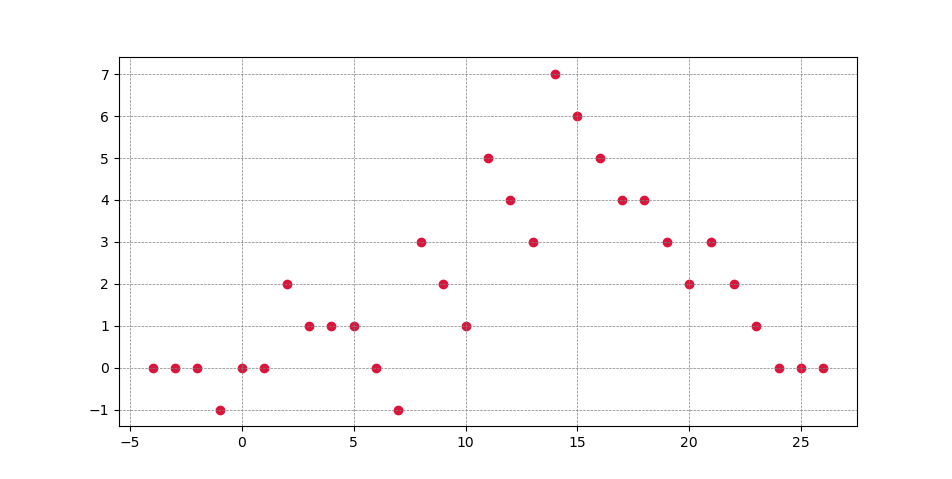
\includegraphics[scale=0.5]{Senial1_28Junio}
\end{figure}
\noindent Una primera idea para facilitar el análisis de esta
puede ser el considerar 
``ventanas'' contiguas de tamaño $z$ y, de alguna forma 
razonable, ``reducir'' la información de la señal contenida 
en estas (esto sin perder
información relevante de la forma
de la original). Podemos agrupar además a una cantidad fija
de ventanas, digamos $s$, en una ventana mayor, para el 
posterior análisis de la señal reducida.


\begin{figure}[H]
	\centering
	\includegraphics[scale=0.5]{Senial2_28Junio}
\end{figure}

\noindent En el ejemplo, observe el trozo de la señal
enmarcado por el tercer subconjunto azul;
a pesar de que esta
sube y baja, el alejarse un poco de esta para verla
``más borrosa'' y tratar de ignorar el ruido 
nos sugiere la forma de una recta de pendiente positiva. 
\begin{figure}[H]
	\centering
	\includegraphics[scale=0.5]{Senial3_28Junio}
\end{figure}

\TODO{aquí una conclusión. Todavía debo trabajar
esta introducción. Debería incluir, explícitamente, 
la analogía del microscopio.}

\section{Análisis local: una resolución}
Lo más sencillo que podemos hacer para analizar
localmente una señal es, a partir
de cierto punto $a \in \IZ$,
considerar a las siguientes
$\mu$ mediciones.


\begin{comment}
1.- Local, un alféizar, una resolución

a: punto de anclaje
\mu: anchura
Señal alféizar: \chi_{a, \mu}
alféizar
ventana
espacio de ventanas V_{a, \mu}
\end{comment}

\begin{defi}
Sean $\mu \in \IN$, $a \in \IZ$. 
Al conjunto de $\mu$ enteros consecutivos
\[
\alpha_{a, \mu}:= [a , a+\mu ) \cap \IZ 
\]
le llamaremos el \textbf{alféizar de anchura $\mu $
y punto de anclaje $a$}.
\footnote{Elegimos el nombre de ``alféizar'' porque, 
para estudiar localmente
una señal, vamos a restringirnos a lo soportado en 
un subconjunto de $\mu$ enteros consecutivos.} \\
\end{defi}

\begin{defi}
Fijado un $\mu \in \IZ^{+}$, a una sucesión de la forma
\[
\chi_{a, \mu}:=\frac{1}{\sqrt{\mu}} \suma{\nu=a}{a+\mu -1}{\delta_{\nu}} \in 
\ell^{2}(\IZ), 
\hspace{0.5cm} a \in \IZ.
\]
le llamaremo \textbf{señal alféizar}.
\end{defi}
Observe que $\chi_{a, \mu}$ no es más que la sucesión de norma uno que es cero
en todos los puntos, menos en
los enteros $\nu$ con $a \leq \nu \leq a + \mu -1$,
donde vale $\frac{1}{\sqrt{\mu}}$; ponemos el factor
$\frac{1}{\mu}$ por cuestiones de normalización, pues lo que
nos interesa es tener una señal unitaria cuyo soporte sea un alféizar
de anchura $\mu$.

\begin{figure}[H]
	\centering
	\includegraphics[scale=0.9]{Senial3_25Mayo}
\end{figure}



\begin{defi} \label{ventanas y espacio de ventanas sobre un alfeizar}
Si $x=(x_{k})_{k \in \IZ}$ es una señal cualquiera,
llamaremos a la señal
\[
x_{|a, \mu}:= 
\suma{\nu=a}{a+\mu -1}{x_{\nu}\delta_{\nu}},
\]
la \textbf{ventana de $x$ en el alféizar $\alpha_{a, \mu}$}. \\ 
Al subconjunto $V_{\alpha , \mu}$ de $\ell^{2}(\IZ)$
que consta de todas las ventanas en el alféizar
$\alpha_{a, \mu}$, o sea, a
\[
V_{\alpha , \mu} := \{ x_{|a, \mu} : x \in \ell^{2} \}
\]
le llamaremos el \textbf{espacio de ventanas en el 
alféizar $\alpha_{a, \mu}$.}
\end{defi}

Observe que $x_{|a, \mu}$ no es más que la señal que
coincide con
$x$ en el alféizar $\alpha_{a,\mu}$ y es cero en los
demás puntos.

\begin{comment}
\begin{figure}[H]
	\centering
	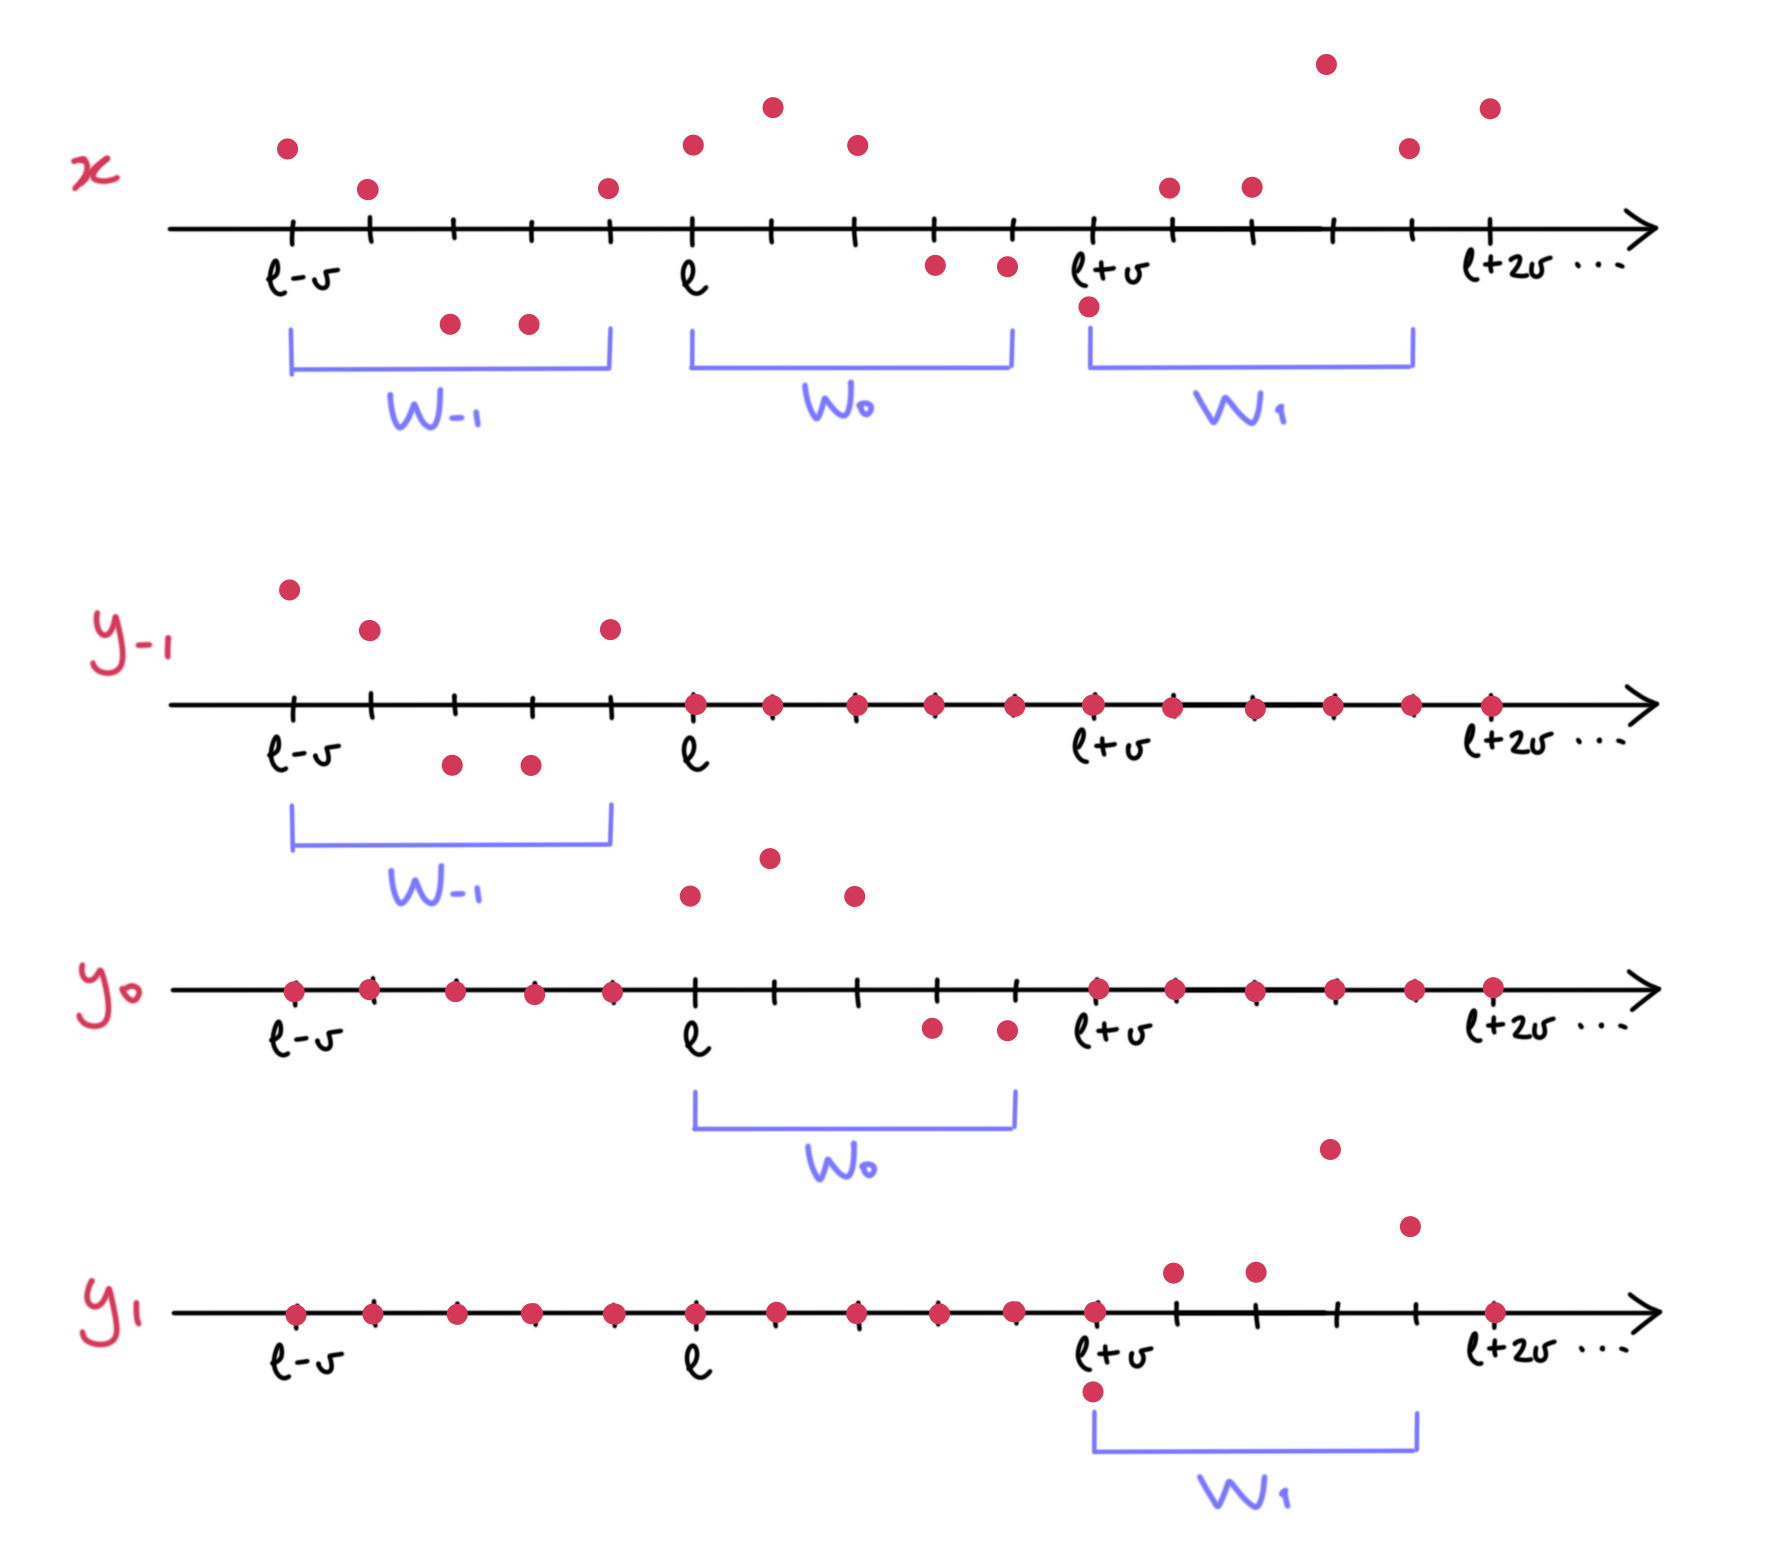
\includegraphics[scale=0.6]{6Junio_2}
	\caption{Una señal arbitraria $x$ y algunas 
	de sus ventanas.}
\end{figure}
\end{comment}

\begin{prop} \label{espacio de ventanas es isometrico a un Rn}
Si $\mu \in \IN$ y $a \in \IZ$, los espacios
\begin{center}
$\IR^{\mu}$
\hspace{0.3cm} y \hspace{0.3cm}
$V_{a, \mu }$
\end{center}
son isométricos.
\end{prop} 
\demostracion 
El subconjunto no vacío $V_{a,\mu}$
de $\ell^{2}(\IZ)$
es claramente cerrado bajo sumas 
y multiplicaciones por escalares,
por lo que es subespacio de $\ell^{2}(\IZ)$ (y por lo 
tanto $\IR-$espacio vectorial en sí mismo). Restringiendo
el producto punto a él, él mismo es un espacio vectorial
con producto punto. 
La función de $\IR^{\mu}$ en 
$V_{a, \mu }$ que a cada vector le asigna 
la señal que es cero en todas partes menos
en el alféizar $\alpha_{a, \mu}$,
donde toma como valores las entradas del vector,
es claramente una isometría. \QEDB



\section{Análisis local: dos resoluciones}
Vamos ahora a plasmar la idea del enfoque esbozada 
en la introducción:
siguiendo con el análisis local de una señal, vamos
a considerar no solo un punto de anclaje $a$
y una anchura $p$, sino también un tercer entero $z$
que divida a $p$ (digamos que $p=zs$), para así
considerar, dentro de $\alpha_{a,p}$, $s$ alféizares
consecutivos de tamaño $z$\footnote{En este
contexto, a atales $s$ alféizares
los denominaremos ``subalféizares''.}, para después sustituir
lo comprendido de una señal en cada uno de estos
por una sola medición promedio.
Así, a diferencia de lo hecho en la sección anterior,
tenemos involucradas \textit{dos} resoluciones $z$ y $p$,
relacionadas por una escala $s$.

Esto nos llevará a construir subespacios de $\ell^{2}(\IZ)$
isomorfos a $\IR^{s}$, para los cuales daremos análogos
de las bases canónica y de Legendre discreta $\cali{L}^{s}$
de $\IR^{s}$. \footnote{Obviamente queremos
usar la teoría desarrollada en 
el Capítulo I
\TODO{\ref{ParteI header}}
para estudiar la morfología
de ventanas de una señal $x \in  \ell^{2}(\IZ)$; 
bien podríamos pensar a una tal ventana como
un vector en $\IR^{s}$ 
(c.f. proposición \ref{espacio de ventanas es isometrico a un Rn})
pero, como queremos desarrollar toda
la discusión en el espacio
de sucesiones $\ell^{2}(\IZ)$, debemos
realizar el trabajo preliminar de dar versiones de los
elementos de la base 
de Legendre discreta $\cali{L}^{s}$ de $\IR^{s}$ en
el espacio $\ell^{2}(\IZ)$, en todos
los alféizares de anchura $p$; hacemos justo eso en
esta sección.}

\begin{center}
\TODO{aquí dibujo?}
\end{center}

\begin{notacion}
Si $z$ es un entero positivo y $s$ un entero mayor a uno,
llamaremos a la pareja ordenada $g=(z,s)$ una \textbf{calibración};
en este contexto, a $z$ le llamaremos el \textbf{enfoque/
resolución/zoom} y a $s$ la \textbf{escala} de la calibración.
Al entero $p:=zs$ le llamaremos \textbf{envergadura/ámbito/scope.}
\end{notacion}

\noindent Dada
una calibración $g=(z,s)$, 
considere un alféizar con punto de anclaje $a$
y anchura $p$. Ya dijimos
cómo en cada subalféizar de tamaño $z$ nos interesa sustituir
lo comprendido en este de una señal $x$ por un solo número,
luego, es natural introducir la siguiente definición.


\begin{defi} 
\label{definición de espacio M a g}
Dados $a \in \IZ$ y $g=(z,s)$
una calibración,
definimos al subespacio $M_{a,g}$
de $\ell^{2}(\IZ)$ como sigue:

\[
M_{a,g}:= span \{ \chi_{a+qz, z}: \hspace{0.2cm} 0 \leq q <s \},
\]
y lo llamamos el \textbf{espacio periferia local}
respecto al punto de anclaje $a$ y calibración $g$.
\end{defi}

\begin{obs} \label{prop: BON1 de Lambda g, k}
Dados $a \in \IZ$ y $g=(z,s)$ una calibración, 
\begin{equation}
\label{eq1: 22Nov}
\{ \chi_{a+qz, z}: \hspace{0.2cm} 0 \leq q <s \}
\end{equation}
es una BON del espacio $M_{a,g}$. Además,
una señal $x$ del espacio es elemento de $M_{a,g}$ si y 
sólo si 
\begin{enumerate}
\item $x_{\nu}=0$ si $\nu < k$ o $\nu \geq k+p$, y
\item Para toda $0 \leq b < s$, si 
$\nu_{1} , \nu_{2} \in [k+bz , k+(b+1)z) $ 
entonces $x_{\nu_{1}}=x_{\nu_{2}}$.
\end{enumerate}
Es decir, $M_{a,g}$ es el conjunto de señales
\begin{itemize}
\item cuyo soporte está contenido en el alféizar
$\alpha_{a, p}$, y

\item que son constantes en cada uno de los $s$ 
subalféizares contiguos de tamaño $z$ que contiene
$\alpha_{a, p}$.
\end{itemize}
\end{obs}



\begin{figure}[H]
	\centering
	\includegraphics[scale=0.8]{Senial4_25Mayo}
	\caption{Ejemplo gráfico de un elemento
	genérico de $M_{a, g}$.
	El que una tal señal evoque la silueta de edificios
	fue la razón por la que elegimos el nombre 
	de ``espacio periferia local'' para este
	tipo de espacios.}
\end{figure}


\begin{cor} \label{cor:dimension de Lambda g,k }
Dada una calibración $g=(z,s)$, para toda $a\in \IZ$
se tiene que
$M_{a,g}$ es un subespacio de $\ell^{2}(\IZ)$
de dimensión $s$.
\end{cor}

Según este último corolario, el espacio
periferia local $M_{a,g}$ es isomorfo a $\IR^{s}$;
a continuación, en términos de la base $\cali{L}^{s}$
de este último espacio construimos una para el primero.


\begin{defi} \label{def: sistema de haar-legendre}
Sean $a \in \IZ$, $g=(z,s)$ una calibración.
Llamaremos a las $s$ señales
\[
\lambda_{a}^{g,d} := \suma{q=0}{s-1}{  \cali{L}^{s,d}_{q+1} 
\chi _{a+qz, z}}, \hspace{0.4cm} \text{con } 0 \leq d \leq s-1 
\hspace{0.2cm} \text{entero}
\]
señales de tipo \textbf{Haar-Legendre}. 
Al subconjunto
\[
\{ \lambda_{a}^{g,d} \hspace{0.2cm} | \hspace{0.2cm} a \in \IZ, 0 \leq d \leq s-1  \}
\]
del espacio $\ell^{2}(\IZ)$  le llamaremos
el \textbf{sistema de Haar-Legendre asociado a la
calibración $g$}.
\end{defi}

Note que la señal
$\lambda_{a}^{g,d}$ es el elemento de $M_{a,g}$
cuyo valor en el $(q+1)-$ésimo subalféizar
de anchura $s$
es igual a la $(b+1)-$ésima entrada del 
vector $\cali{L}^{s,d}$ de $\IR^{s}$ multiplicada
por $\frac{1}{\sqrt{z}}$; multiplicamos por esta constante
simplemente para que las señales resultantes tenga norma uno.
Lo importante es que ellas se definieron a partir de 
los elementos de $\cali{L}^{s}$; recuerde que esta base
nos importa pues dimos 
interpretaciones geométricas de nuestro interés sobre
lo que significa ser elemento de los subespacios $W_{0}$,
$W_{1}$ y $W_{2}$
de $\IR^{s}$ que generamos
a partir de los primeros tres elementos de $\cali{L}^{s}$. 



\begin{figure}[H]
	\centering
	\includegraphics[scale=0.8]{24Oct_1}
	\caption{En la figura se ilustran las gráficas de las señales
	de $\cali{L}^{4}$ y las señales de tipo Haar-Legendre
	asociadas al punto de anclaje $-2$ y a la calibración
	$g=(3,4)$.}
\end{figure}

\begin{obs} \label{obs: senales de haar-legendre de grado cero son constantes}
Para cualesquiera $a \in \IZ$ 
y $g=(z,s)$,
\[
\lambda_{a}^{g,0}= \left( \frac{1}{s}, \ldots ,\frac{1}{s} \right).
\]
\end{obs}

\begin{prop} \label{prop: BON de M a g dual a la de Legendre discreta de Rs}
Dados $a \in \IZ$ y una calibración $g=(z,s)$, 
el subconjunto 
\[
\{ \lambda_{a}^{g,d} \hspace{0.2cm} | \hspace{0.2cm} 0 \leq d \leq s-1 \}
\]
del espacio $M_{a,g}$
es una BON de este. 
\end{prop}
\begin{dem} Por lo establecido en 
el corolario \ref{cor:dimension de Lambda g,k },
si demostramos que las $s$ señales 
del conjunto propuesto
son unitarias
y ortogonales entre sí, acabamos. \\
Usando la bilinealidad del producto punto y el que 
$\{ \chi_{a+qz, z}: \hspace{0.2cm} 0 \leq q <s \}$
sea una BON del espacio $M_{a,g}$ (c.f.
observación \ref{prop: BON1 de Lambda g, k}),
tenemos que, para $0 \leq d_{1}, d_{2} \leq s-1$
enteros cualesquiera,
\begin{align*}
\langle \lambda_{a}^{g,d_{1}} , \lambda_{a}^{g,d_{2}} \rangle 
& = \langle \suma{b=0}{s-1}{\cali{L}_{b+1}^{s,d_{1}} \chi _{a+bz,z} },
 \suma{c=0}{s-1}{\cali{L}_{c+1}^{s,d_{2}} \chi _{a+cz,z} } \rangle \\
& =\suma{b=0}{s-1}{\langle \cali{L}_{b+1}^{s,d_{1}} \chi _{a+bz,z},
\cali{L}_{b+1}^{s,d_{1}} \chi _{a+bz,z} \rangle }\\
& = \suma{b=0}{s-1}{\cali{L}_{b+1}^{s,d_{1}} \cali{L}_{b+1}^{s,d_{2}}} \\
& =\langle \cali{L}^{s,d_{1}} , \cali{L}^{s,d_{2}} \rangle,
\end{align*}
\noindent 
donde los productos punto son los del espacio 
$\ell^{2}(\IZ)$ menos el último, que es el de 
$\IR^{s}$; puesto que $\cali{L}^{s}$ es una
base ortonormal de $\IR^{s}$, concluimos 	que este 
último es igual a $\delta_{d_{1}, d_{2}}$.

\QEDB
\end{dem}

Más adelante, será de utilidad considerar al subespacio
de $M_{a,g}$ que consta de todos los elementos
de $M_{a,g}$ que no son constantes en todo el alféizar
$\alpha_{a, p}$; según la observación 
\ref{obs: senales de haar-legendre de grado cero son constantes}
y la proposición
\ref{prop: BON de M a g dual a la de Legendre discreta de Rs},
para definir a este espacio basta con no considerar a la 
señal de Haar-Legendre de grado cero.

\begin{defi}
\label{espacios N_{a,g}} Dados $a \in \IZ$ y $g=(z,s)$
una calibración, definimos al subespacio $N_{a,g}$
de $M_{a,g}$ como sigue:
\[
N_{a,g}:= span \{ \lambda_{a}^{g,d}: 0 < d < s \}.
\]
Llamamos a este el \textbf{espacio local bifocal}
respecto al punto de anclaje $a$ y calibración $g$.
\end{defi} 


\begin{obs} \label{obs: espacio N a g}
Dados $a \in \IZ$ y $g=(z,s)$
una calibración,
\[
N_{a,g}= span\{ \chi_{a+qz, z} : 0 \leq q \leq s-1 \} \boxminus span \{ \chi_{a, p}\}.
\]
\end{obs}

\begin{prop}
Si $x= \suma{q=0}{s-1}{c_{q}\chi_{a+qz,z}}$ es un elemento
del espacio $M_{a,g}$, entonces $x \in N_{a,g}$ si y sólo si
$\suma{q=0}{s-1}{c_{q}}=0$.
\end{prop}
\begin{dem}
En efecto, según la observación 
\ref{obs: espacio N a g}, $x$ es elemento de $N_{a,g}$
si y sólo si $<x, \chi_{a,p}>=0$, o sea, si y sólo si
\[
0=<x, \chi_{a,p}>=
\suma{q=0}{s-1}{c_{q}<\chi_{a+qz,z}, \chi_{a,p}>}
=\suma{q=0}{s-1}{c_{q}\left( \frac{z}{\sqrt{z}} \right)}
=\left( \frac{z}{\sqrt{z}} \right)\suma{q=0}{s-1}{c_{q}}.
\] 
$\QEDB$
\end{dem}

\noindent
Terminamos esta sección
con algunos comentarios.
\begin{itemize}
\item Fijados $g=(z,s)$ y $a \in \IZ$, hemos
definido a un subespacio $M_{a,g}$ de $\ell^{2}(\IZ)$
isométrico a $\IR^{s}$;
la base \eqref{prop: BON de M a g dual a la de Legendre discreta de Rs}
es para el espacio $M_{a,g}$ lo que la base de Legendre
discreta $\cali{L}^{s}$ (definida en 
\ref{def: base de Legendre discreta}) es para $\IR^{s}$,
y la base \eqref{eq1: 22Nov} de $M_{a,g}$ es para
este espacio lo que la base canónica de $\IR^{s}$
es para este último espacio.

\item Nos interesa este espacio $M_{a,g}$
y sus dos BON descritas para el análiss
local de una señal; 
dada $x \in \ell^{2}(\IZ)$,
lo que haremos, a grandes rasgos,
será restringirnos a un alféizar $\alpha_{a, p}$,
o sea, considerar a la ventana
$x_{|a, p}$, para luego, via el cálculo de
ciertos productos puntos\footnote{c.f.
\TODO{ref}, más adelante.}, realizar un proceso de 
síntesis; la información comprendida en uno de los $s$
subalféizares contiguos contenidos
en $\alpha_{a,p}$ de tamaño $z$ será sustituida
por una sola medición.
Realizado este proceso de síntesis, en base a coeficientes
calculados a partir de la base 
\eqref{prop: BON de M a g dual a la de Legendre discreta de Rs}, 
vamos a realizar un análisis morfológico de la señal
resultante. 
\end{itemize}

\begin{figure}[H]
	\centering
	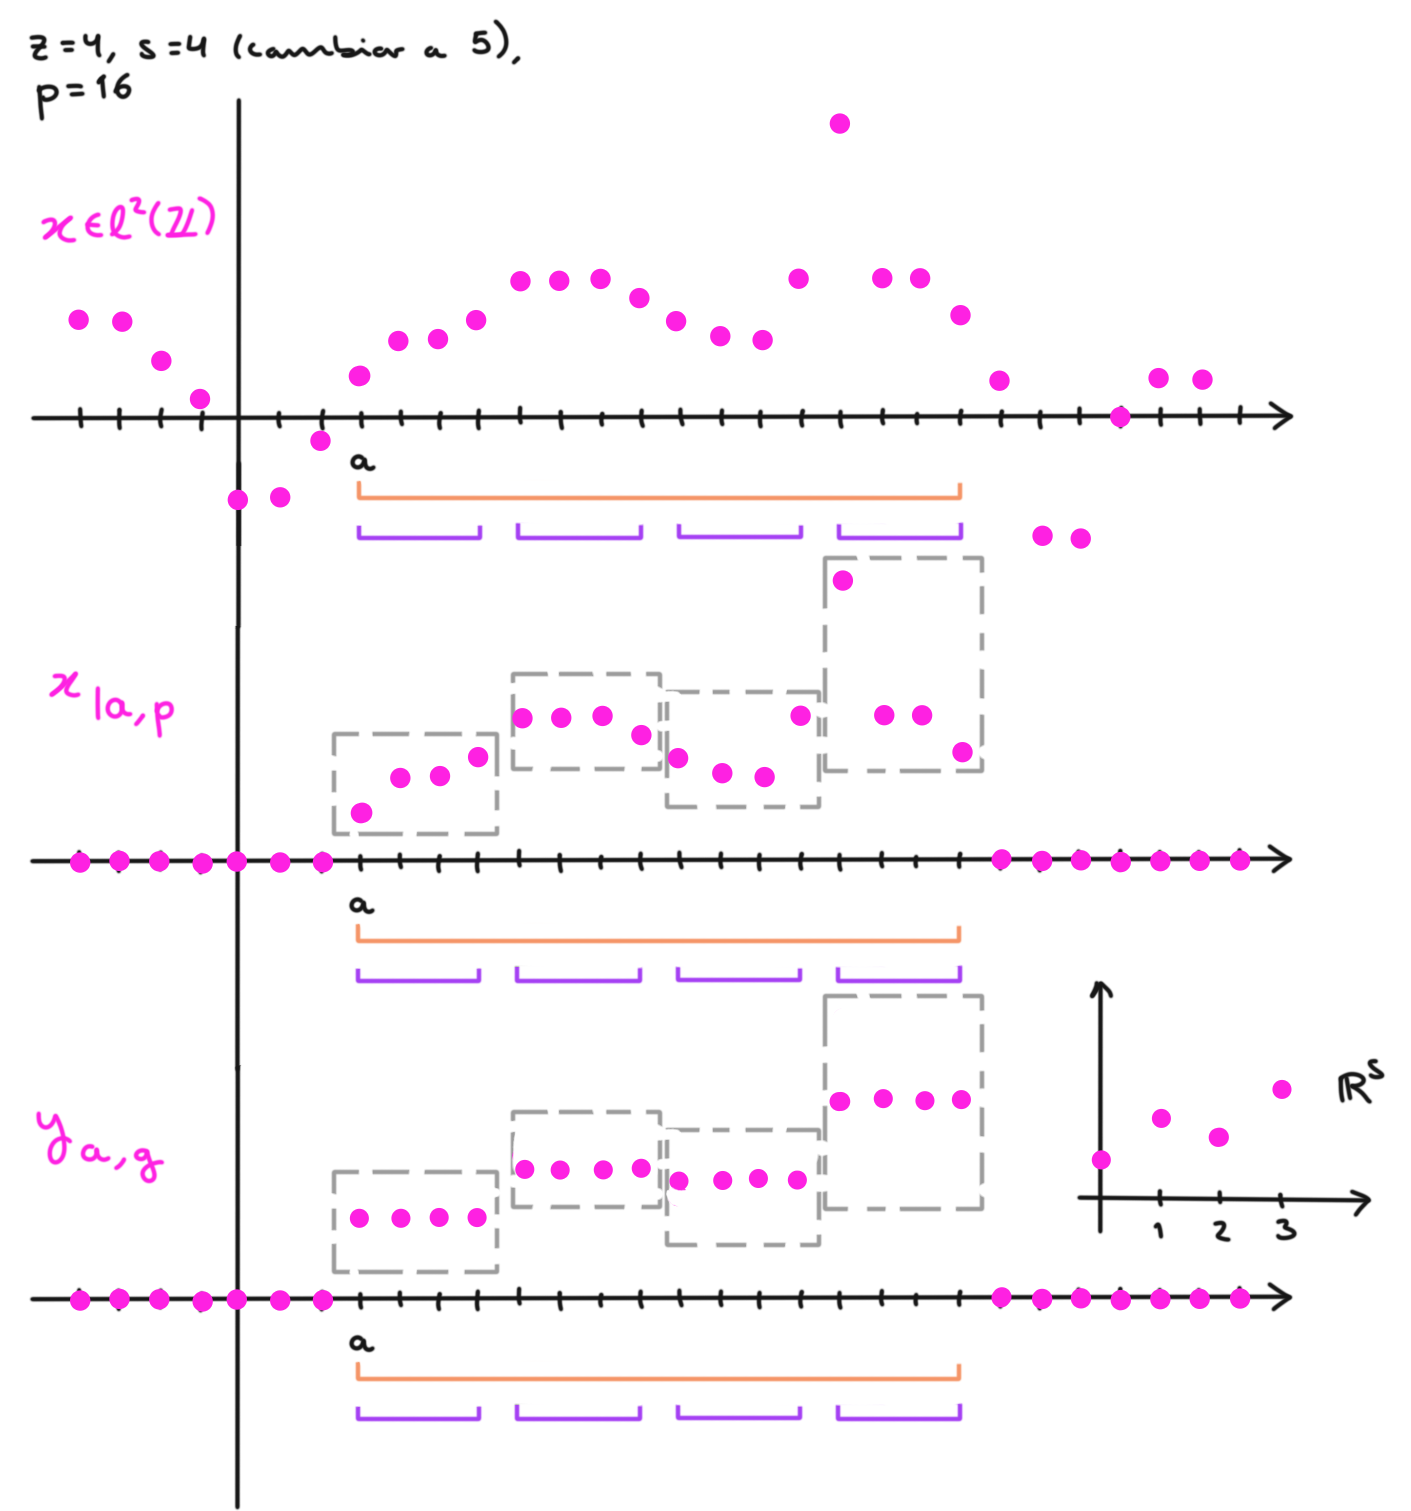
\includegraphics[scale=0.9]{22Nov_1}
	\caption{Ejemplo gráfico para cuando $z=s=4.$}
\end{figure}




\begin{comment}
2.- Local, dos resoluciones 
zoom, escala, ámbito, calibracion.

Espacios periferia locales: M_{a,g}
Espacios bifocales locales: N_{a,g}
\end{comment}


\section{Análisis global: una resolución}

\begin{notacion}
Por $\phi$ denotaremos a un número entero
fijado a partir del cual partir a $\IZ$
con alféizares de anchura $\mu$.
Acostumbraremos
llamar a $\phi$ un \textbf{desfase}.
\end{notacion}
\begin{center}
\TODO{esquema.}
\end{center}

Queremos seguir usando alféizares 
a partir de las cuales formar ventanas
de una señal, para así, por medio
de estos primeros objetos, estudiar el segundo,
pero como ahora queremos un análisis global, debemos
considerar no un solo alféizar, sino una colección
disjunta de estos.

\begin{obs} \label{obs:particiones con alféizares}
Si $\phi \in \IZ$ y $\mu \in \IN$, los alféizares
de anchura $\mu$ y punto de anclaje de la forma
\[
a_{q}= \phi +q \mu, \hspace{0.4cm} q \in \IZ
\]
conforman una partición de $\IZ$,
que denotamos por 
\[
\cali{A}_{\phi , \mu}
\]
y llamamos un \textbf{teselado}.
\end{obs}

\begin{obs} \label{obs: sobre sufalfeizares}
Sean $\mu_{1}, \mu_{2} \in \IN$, $\phi \in \IZ$.
Si $\mu_{1}| \mu_{2}$, digamos $\mu_{1} s = \mu_{2}$, 
entonces todo elemento de la partición $\cali{A}_{\phi, \mu_{2}}$
contiene exactamente $s$ elementos de 
la partición 
$\cali{A}_{\phi, \mu_{1}}$.
\end{obs}
Recuerde que,
en el contexto de la observación anterior, 
acordamos llamar
a los elementos de $\cali{A}_{\phi, \mu_{1}}$ ``subalféizares''.

\noindent
Ahora que contamos con un teselado, podemos considerar ventanas
con soportes disjuntos de una señal $x$
(\textbf{proceso de análisis}); parece razonable
pensar que a partir de estas resulta sencillo recuperar
a la señal original 
(\textbf{proceso de síntesis}). 
Comprobamos que esto ocurre en la
siguiente proposición.

\begin{prop} \label{prop: descomposicion de una señal en ventanas}
Sean $\phi \in \IZ $, $\mu \in \IN$.
Sea $x=(x_{k})_{k \in \IZ} \in \ell^{2}(\IZ)$. 
Si
\[
y_{q}:= x_{|\phi + q \mu, \mu} , \hspace{0.7cm}
q \in \IZ,
\]
entonces
\[
x=\suma{q \in \IZ}{}{y_{q}}.
\]
\end{prop}
\begin{dem}

Si $\sigma : \IN \longrightarrow \IZ$ es una biyección
\footnote{Que, en el contexto de la demostración, 
se usa para enumerar los elementos del teselado 
$\cali{A}_{\phi, \mu}$.}
cualquiera,
demostremos que
\[
x = \limite{N \rightarrow \infty }{ \suma{n=1}{N}{y_{\sigma (n)}}}
\hspace{0.2cm} \text{ en }
\ell^{2}(\IZ).
\]

\noindent 
El soporte de la señal $y_{q}$ es el alféizar
$W_{q}:= \alpha_{ \phi + q \mu, \mu}$;
haciendo variar $q$ en $\IZ$,
según la observación \ref{obs:particiones con alféizares},
estos forman una partición de $\IZ$; puesto que con
la sucesión $\sigma$ enumeramos a estos alféizares
$W_{q}=W_{\sigma(n)}$, 
en base a ella podemos construir una biyección
$\psi : \IN \longrightarrow \IZ $ para enumerar a los enteros
respetando el orden en el que $\sigma$ enumera 
a los alféizares como sigue: \\

Sea $n \in \IN$. Si $a_{n}$ es el único natural tal que
$(a_{n}-1)\mu +1 \leq n \leq a_{n} \mu $, entonces
\[
\psi (n) := l + (\sigma (n) -a_{n}+1) \mu + n-1.
\]

Como $x \in \ell^{2}(\IZ)$, la serie
$\suma{n=1}{\infty}{|x_{\psi(n)}|^{2}}$ es convergente.

\begin{figure}[H]
	\centering
	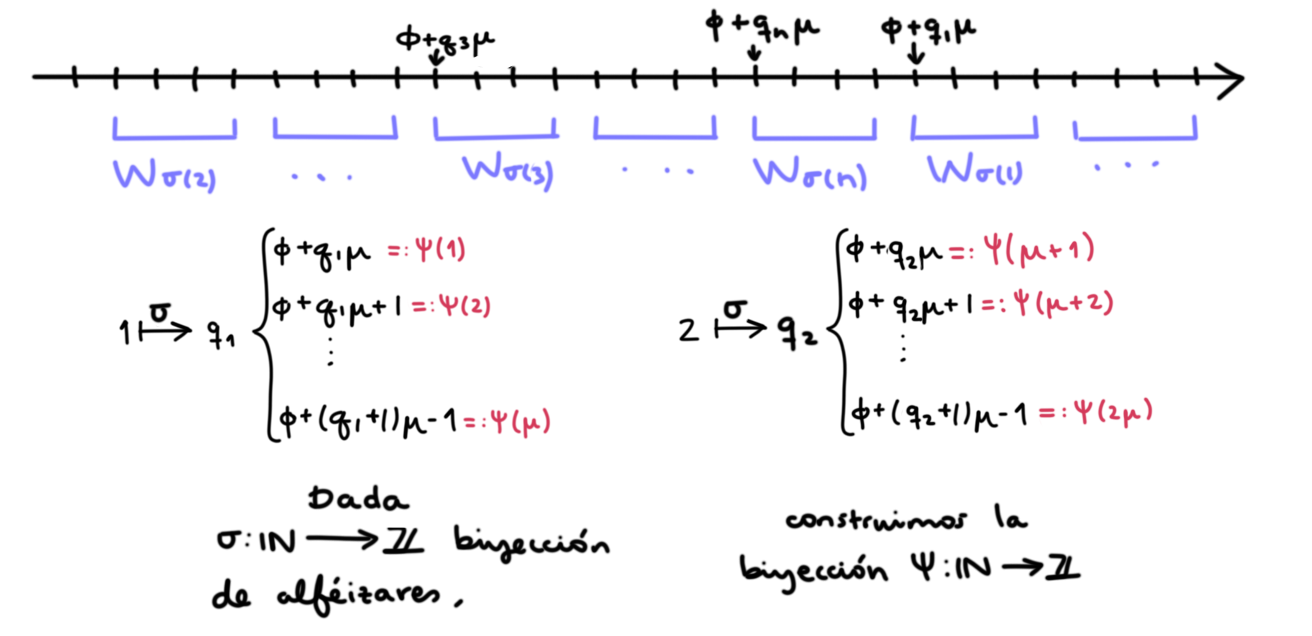
\includegraphics[scale=0.8]{10Junio}
\end{figure}


Ahora bien, si para $N \in\IN$
definimos a la señal $r_{N}$ como
\[
r_{N}:= x- \suma{n=1}{N}{y_{\sigma (n)}},
\]
esta es la señal que es cero en los alféizares
\[
W_{\sigma(1)}, \ldots , W_{\sigma(n)}
\]
y coincide con $x$ en los demás; así,
los cuadrados de las normas de las señales $r_{N}$
son colas de la serie convergente 
$\suma{n=1}{\infty}{|x_{\psi(n)}|^{2}}$, luego,
las normas de las señales $r_{N}$ convergen
a cero conforme $N \rightarrow \infty$, o sea, la sucesión 
$$\left( \suma{n=1}{N}{y_{\sigma (n)}} \right)_{N \in \IN}$$
en efecto converge a la señal $x$
en el espacio $\ell^{2}(\IZ)$.
\QEDB
\end{dem}


\noindent Recuerde que la idea es sustituir las mediciones
encerradas en cada subalféizar $\alpha_{a+qz,z}$ por una sola
(reduciendo así $p$ mediciones originales a sólo $s$).
El vector cuyas entradas son estas mediciones es
\[
(x(a+qz), \ldots , x(a+qz+z-1)).
\]


\begin{prop} \textbf{(proceso de modificación de una señal)}
\label{prop: modificacion senial}
\TODO{revisar!}
\footnote{Note que
la formulación de esta proposición no depende de los parámetros
$s$ y $p$ de una calibración, sólo de $z$ y del
punto de anclaje $a$ escogido.} Sean 
$a \in\IZ$, $z \in \IZ^{+}$.
Sea $x \in \ell^{2}(\IZ)$ una señal cualquiera. Si
por $y_{x,q}$ denotamos al producto punto
\[
\langle (x(l+qz), \ldots , x(l+qz+z-1)) , 
 \frac{1}{\sqrt{z}} (1, \ldots ,1) \rangle,  
\hspace{0.5cm} q \in \IZ ,
\]
entonces la función 
\begin{align*}
y_{x}: & \IZ \longrightarrow \IR \\
q & \mapsto y_{x,q}
\end{align*}
es elemento de $\ell^{2}(\IZ)$.
\end{prop}
\begin{dem}
\TODO{revisar!}
Para toda $q \in \IZ$, por la desigualdad de Cauchy-Schwarz
(teorema \ref{Teo:CauchySchwarz})
en $\IR^{z}$,
\begin{align*}
|y_{x,q}|^{2} & \leq ||(x(l+qz), \ldots , x(l+qz+z-1))||^{2} 
\cdot 1 \\
& = |x(l+qz)|^{2} + \cdots + |x(l+qz+z-1))|^{2};
\end{align*}
\noindent
observando que si $q_{1} \neq q_{2}$ los índices
involucrados para calcular $|y_{x, q_{1}}|$ y 
$|y_{x, q_{2}}|$ son todos distintos entre sí
(observación \ref{obs:particiones con alféizares}), tenemos que,
si $\sigma : \IN \longrightarrow \IZ$ 
es una biyección cualquiera,
las sumas parciales $\suma{n=1}{N}{|y_{x, \sigma(n)}|^{2}}$
están acotadas superiormente por
la suma de la serie $\suma{n=1}{\infty}{|x_{\sigma(n)}|^{2}}$
que, por ser $x$ elemento de $\ell^{2}(\IZ)$, es finita;
así,
por el criterio de acotación, la serie 
$\suma{n=1}{\infty}{|y_{x, \sigma(n)}|^{2}}$ converge, o sea,
$y \in \ell^{2}(\IZ)$.
\QEDB
\end{dem}


\begin{defi}
A la señal de la proposición anterior
le llamaremos la \textbf{reducción
de $x$ respecto a $z$ y al desfase $\phi$}. 
\end{defi}


\begin{figure}[H]
	\centering
	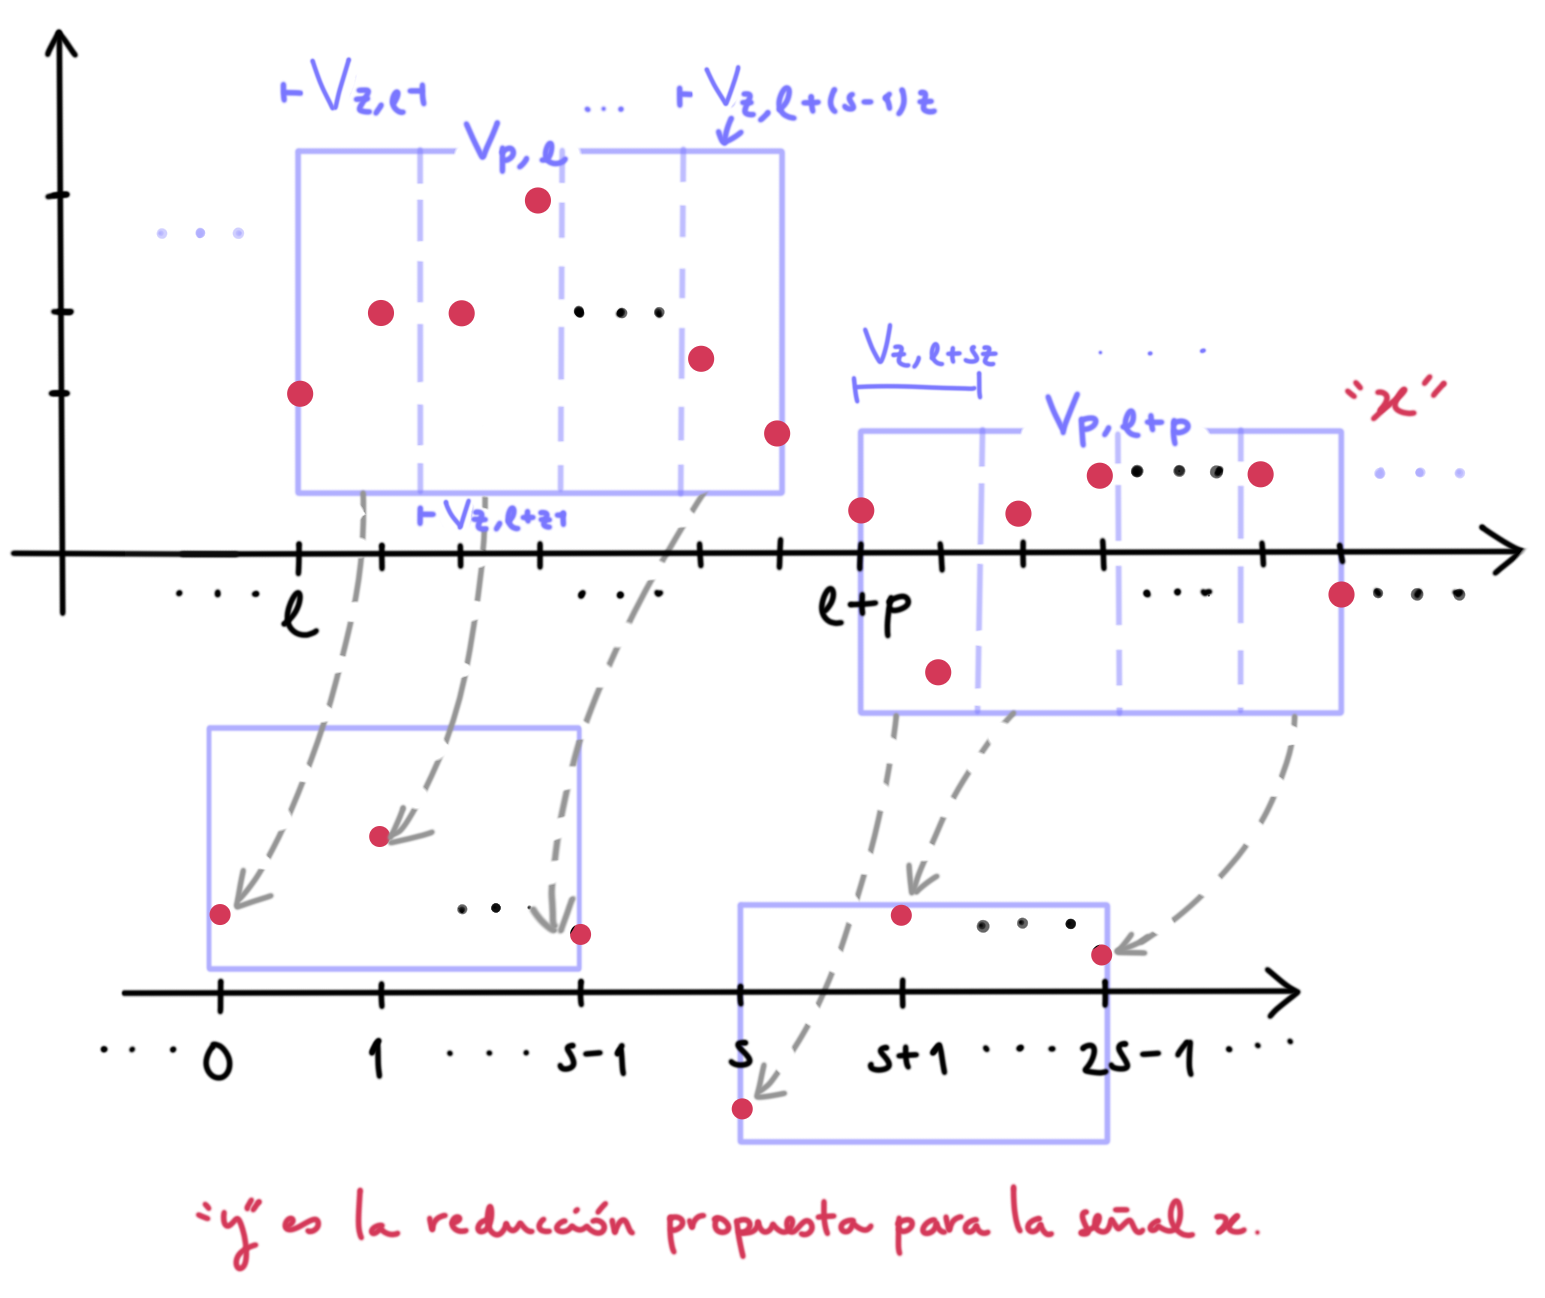
\includegraphics[scale=0.5]{2Junio_1}
	\caption{Ilustración del proceso de reducción propuesto.
	\TODO{Esto en realidad es ligeramente diferente a lo puesto en otra
	imagen. ¿qué es lo que haremos al final? Creo que no lo 
	plasmado en esta imagen, sino en la anterior.}}
\end{figure}

En vistas de la forma de las señales
que resultan del proceso 
de modificación expuesto en 
\ref{prop: modificacion senial}, claro que conviene
considerar al subconjunto de $\ell^{2}(\IZ)$
que consta de señales de esta forma;
como veremos, 
este es un subespacio cerrado 
de $\ell^{2}(\IZ)$.
Antes de dar una formulación para él, establezcamos
una sencilla proposición.

\begin{prop}
\label{prop: las chi con dominio particion por ventanas forman un sist. ort.}
Fijados un 
$\phi \in \IZ$ y un 
$\mu \in \IZ^{+}$,
\begin{equation}
\label{eq2: 22Nov}
\{ \chi_{\phi + q\mu, \mu}, \hspace{0.2cm} | \hspace{0.2cm} 
q \in \IZ \}
\end{equation}
es un subconjunto ortonormal y numerable
de $\ell^{2}(\IZ)$.

\end{prop}
\begin{dem}
El que las señales $ \chi_{\phi + q\mu, \mu}$ tengan norma uno se 
cumple por definición. El soporte de luna señal
$\chi_{a, \mu}$ es el alféizar $\alpha_{a, \mu}$,
luego, dos señales del conjunto \eqref{eq2: 22Nov}
distintas entre sí tienen soportes disjuntos
(c.f. observación \ref{obs:particiones con alféizares}), 
luego, son trivialmente ortogonales entre sí.
 \QEDB
\end{dem} 


\begin{defi} 
Dados $\phi \in \IZ$ y $\mu \in \IN$,
llamaremos al subespacio cerrado de $\ell ^{2}(\IZ)$
\begin{align*}
X_{\phi, \mu } :=  &\overline{span} \{ \chi_{a, \mu} | a \equiv \phi
\hspace{0.2cm} (mod \hspace{0.1cm} \mu) \} \\
=  &\overline{span} \{ \chi_{\phi +q \mu, \mu} | q \in \IZ \} 
\end{align*}
el \textbf{espacio periferia de 
desfase $\phi$ y
anchura $\mu$}.
\end{defi}


\noindent Establecemos unos resultados sencillos sobre estos espacios; 
el primero nos da un criterio de pertenencia.

\begin{teo}
\label{teo:caracterizacion espacios periferia}
\textbf{(caracterización de los espacios periferia):}
Sean $\mu \in \IN$, $\phi \in \IZ$. Las proposiciones
\begin{itemize}
\item $x \in X_{\phi, \mu}$ , y
\item existe $a=(a_{q})_{q \in \IZ} \in \ell ^{2}(\IZ)$
tal que 
$x=\suma{q\in \IZ}{}{a_{q}\chi_{\phi+q \mu ,\mu}}$
\end{itemize}
son equivalentes, es decir,
una señal $x$ es elemento de $X_{\phi, \mu}$ si y sólo si

\begin{enumerate}
\item en el alféizar $W_{q}:=\alpha_{\phi + q \mu, \mu}$ 
la señal $x$ es constante
(digamos que toma en todos los puntos de este el valor
$\frac{a_{q}}{\sqrt{\mu}}$), y

\item la serie $\suma{q \in \IZ}{}{|a_{q}|^{2}}$ es convergente.
\end{enumerate}

\end{teo}
\begin{dem} Denotemos por $X$ al espacio
\[
span \{ \chi_{k, \mu} | k= \phi + q \mu, 
\hspace{0.2cm} q \in \IZ \}.
\]
Según nuestra definición,
\begin{center}
$x \in $ si y sólo si $x$ es punto
de cerradura de $X$;
\end{center}

\noindent
como la topología del espacio $\ell^{2}(\IZ)$
está inducida por una métrica, podemos reescribir esta
última condición como

\begin{center}
$x \in X_{\phi, \mu}$ si y sólo si existe una sucesión $(x_{n})_{n \in \IN}$
en $X$ que converge a $x$.
\end{center}
\noindent 
Denotemos a la señal $x_{n}$, el $n-$ésimo elemento de una tal
sucesión, por $(x_{n,m})_{m \in \IZ}$.

\begin{itemize}
\item[$\Rightarrow$ )] Sea $(x_{n})_{n \in \IN}$ una sucesión
en $X$ tal que 
\[
\limite{n \rightarrow \infty}{x_{n}}=x,
\]
donde $x=(x_{m})_{m \in \IZ} \in \ell^{2}(\IZ)$. \\
Es fácil ver que la convergencia en $\ell^{2}(\IZ)$
implica la convergencia puntual: para toda $m \in \IZ$,
\begin{align*}
0 \leq |x_{n,m}-x_{m}|^{2}  &\leq \suma{m=1}{\infty}{|x_{n,m}-x_{m}|^{2}} \\
& =d(x_{n},x)^{2} \rightarrow 0 \hspace{0.5cm} \text{conforme}
\hspace{0.2cm} n \rightarrow \infty,
\end{align*}
es decir,
\[
\forall m \in \IZ: \hspace{0.5cm} \limite{n \rightarrow \infty}{x_{n,m}}=x_{m}.
\]

Sea ahora $q \in \IZ$. 
Por ser, para toda $n \in \IN$, $x_{n}$ elemento de $X$, esta señal
es constante en cualquier alféizar
$W_{q}=\alpha_{\phi + q \mu , \mu}= \{ \phi+q \mu,\phi+q \mu+1,\ldots ,\phi +2\mu -1 \} $,
luego, las sucesiones en $\IR$
\[
(x_{n, \phi + q\mu})_{n \in \IN}, \ldots , (x_{n, \phi + 2\mu-1})_{n \in \IN}
\]
son todas iguales entre sí, por lo tanto, sus límites, que
son los números
\[
x_{\phi + q \mu}, \ldots , x_{\phi +2\mu -1},
\]
son trivialmente iguales entre sí, es decir, la señal $x$
es constante en el alféizar $A_{q}$. Si por $a_{q}$
denotamos el valor que toma $x$ en $W_{q}$,
tenemos que el cuadrado de la norma de $x$ es
\[
\suma{v \in \IZ}{}{\mu |a_{q}|^{2}};
\]
de la convergencia de esta serie se deduce la de
la serie $\suma{v \in \IZ}{}{|a_{\nu}|^{2}}$.

\item[$\Leftarrow$ )] El que existan 
$\phi : \IN \longrightarrow \IZ $ biyección y
$\{ a_{\nu} \}_{\nu \in \IZ}$ sucesión real tales que
\begin{center}
$x= \limite{N \rightarrow \infty }{ x_{N} }$,
donde $x_{N}= \suma{n=1}{N}{a_{\phi(n)}\chi_{\phi + \mu \phi(n),\mu }}$
\end{center}

ya expone a $x$ como elemento de la cerradura de $X$,
pues cada $x_{N}$ es combinación lineal finita de señales
de la forma
\[
\chi_{k, \mu},\hspace{0.3cm} \text{con} \hspace{0.2cm} 
k \equiv \phi \hspace{0.2cm} (mod \hspace{0.2cm} \mu),
\]

i.e. elemento del espacio $X$.
\end{itemize}
\QEDB
\end{dem}



\begin{figure}[H]
	\centering
	\includegraphics[scale=0.8]{29Mayo_2}
	\caption{Elemento genérico de $X_{\mu , l}$.
	\TODO{cambiar notación.}}
\end{figure}

\begin{obs} \label{prop: BON para espacios periferia}
$\{ \chi_{\phi + q \mu, \mu} | q \in \IZ\}$
es BON del espacio periferia $X_{\phi, \mu}$.
\end{obs}



\begin{prop} \label{prop: ventanas son constantes a la primera de Haar-Legendre}
Sean $\phi \in \IZ$, $\mu \in \IN$.
Si $x \in X_{\phi, \mu}$ entonces, para toda $q \in \IZ$,
la ventana $y_{q}:= x_{|\phi+q\mu, \mu}$ 
de $x$ es múltiplo
escalar
de la señal 
de tipo Haar-Legendre $\lambda_{\phi+q\mu}^{g,0}$.
\TODO{no sería $x \in X_{\phi, p}$????}
\end{prop}
\begin{dem}
Sólo observe que tanto las señales
$y_{q}$ como $\lambda_{\phi+q\mu}^{g,0}$
tienen sus soportes contenidos en 
el alféizar
$\alpha_{\phi+q\mu, \mu}$ 
y son constantes en este (lo primero
por pertenecer $x$ al espacio periferia y por
el teorema 
\ref{teo:caracterizacion espacios periferia}, 
lo segundo por definición de
$\lambda_{\phi+q\mu}^{g,0}$).
\QEDB
\end{dem}

Terminamos esta sección estableciendo
algunos resultados sobre espacios periferia.

\begin{lema}
\label{teo:hechos espacios periferia}
Sean $\mu, \mu_{1}, \mu_{2} \in \IN$, $\phi, \phi_{1}, \phi_{2} \in \IZ$.
\begin{enumerate}
\item $X_{\phi, 1}= \ell^{2}(\IZ) $ 
\item (Fijando una anchura y variando el desfase):
\begin{center}
$X_{\phi_{1}, \mu} \cap X_{\phi_{2}, \mu} = \{ 0 \} $
si  $\phi_{1} \not\equiv \phi_{2} (mod \hspace{0.2cm} \mu)$,
\end{center}

\begin{center}
$X_{\phi_{1}, \mu } = X_{\phi_{2}, \mu} $
si $\phi_{1} \equiv \phi_{2} (mod \hspace{0.2cm} \mu)$.
\end{center}
Así, hay exactamente $\mu$ espacios 
periferia de anchura $\mu$, es decir,
cualquier espacio $X_{\phi, \mu }$ será uno de entre
los espacios
\[
X_{\mu , 0}, X_{\mu , 1} , \ldots , X_{\mu , \mu -1}.
\]

\item
$ X_{\phi_{1}, \mu} \not\perp X_{\phi{2}, \mu} $.


\item Si
$\mu_{1} | \mu_{2} $ y $\phi_{1} \equiv \phi_{2} (mod \hspace{0.2cm} \mu_{1})$,
entonces
$X_{\phi_{2}, \mu_{2}} \subseteq X_{\phi_{1}, \mu_{1}} $, 
en particular, 

\item (Fijando un desfase y variando la anchura):
 si $\mu_{1} | \mu_{2} $  entonces 
$X_{\phi, \mu_{2}} \subseteq X_{\phi, \mu_{1}} $.
\end{enumerate}
\end{lema}
\begin{dem}
Siendo obvia la demostración del primer punto, pasamos
a la del segundo. 
\begin{itemize}
\item[2)] Digamos primero que $\phi_{1} \not\equiv \phi_{2} (mod \hspace{0.2cm} \mu)$.
Como $X_{\phi_{1}, \mu}$ y $X_{\phi_{2}, \mu}$ son ambos
espacios vectoriales, su intersección es no vacía; 
sea entonces $x$
una señal que pertenece a ambos
espacios. Si mostramos que $x$ es constante,
puesto que la única sucesión constante elemento de $\ell^{2}(\IZ)$
es la sucesión cero, podremos concluir lo deseado. Observe que basta
demostrar que en los puntos comprendidos en 
dos alféizares contiguos
$\alpha_{\phi_{1} +q \mu, \mu}$ y $\alpha_{\phi_{1} +(q+1) \mu, \mu}$
la función
$x$ vale lo mismo. Puesto que 
$\phi_{1} \not\equiv \phi_{2} (mod \hspace{0.2cm} \mu)$, existe un
alféizar $\alpha_{\phi_{2} + r \mu, \mu}$ que contiene puntos
tanto de $\alpha_{\phi_{1} +q \mu, \mu}$
como de $\alpha_{\phi_{1} +(q+1) \mu, \mu}$; por
pertenecer $x$ a $\alpha_{\phi_{2} + r \mu, \mu}$
$x$ es constante en los puntos de este alféizar. De 
esto deducimos, como queríamos, que $x$ toma 
el mismo valor en los dos alféizares 
$\alpha_{\phi_{1} +q \mu, \mu}$ y $\alpha_{\phi_{1} +(q+1) \mu, \mu}$.

\begin{figure}[H]
	\centering
	\includegraphics[scale=0.8]{30Mayo_1}
	\caption{\TODO{Cambiar notación.}}
\end{figure}


En el caso $\phi_{1} \equiv \phi_{2} (mod \hspace{0.2cm} \mu)$,
tenemos que las particiones de los enteros
formados al considerar los alféizares de ancho
$\mu$ y puntos de anclaje $\phi_{1}$
y $\phi_{2}$ son las mismas, por lo que los espacios
$X_{\phi_{1}, \mu}$ y $X_{\phi_{2}, \mu}$ coinciden
trivialmente.

\item[3)] Según el segundo punto
de este teorema, si $\phi_{1}$
y $\phi_{2}$ son congruentes módulo $\mu$, los espacios
$X_{\phi_{1}, \mu}$ y $X_{\phi_{2}, \mu}$ coinciden, luego,
no pueden ser ortogonales entre sí. En caso contrario,
considere a los alféizares
$\alpha_{\phi_{1} +q \mu, \mu}$
y $\alpha_{\phi_{2} + r  \mu, \mu,}$ como en la demostración
del segundo punto;
digamos que estos tienen $b>0$
puntos en común. Como estos son los soportes
de las señales $\chi_{\phi_{1}+q \mu, \mu}$
y $\chi_{\phi_{2}+k \mu, \mu}$, el producto punto
de estas señales es $\frac{b}{\mu }>0$;
hallamos así una señal de 
$X_{\phi_{1}, \mu}$ que no 
es ortogonal a una señal de  $X_{\phi_{2}, \mu}$.

\item[4) ]
Digamos que $\mu_{2}= \nu \mu_{1}$. \\
Consideremos a las particiones de $\IZ$
\begin{center}
 $\cali{A}_{\phi_{1}, \mu_{1}} = \{\alpha_{k, \mu_{1}} \hspace{0.2cm} |
\hspace{0.2cm} k \equiv \phi_{1} (mod \hspace{0.2cm} \mu_{1}) \} $
y 
$\cali{A}_{\phi_{2}, \mu_{2}} = \{\alpha_{k, \mu_{2}} \hspace{0.2cm} |
\hspace{0.2cm} k \equiv \phi _{2} (mod \hspace{0.2cm} \mu_{2}) \} $.
\end{center}

Si demostramos que todo elemento de $\cali{A}_{\phi_{1}, \mu_{1}}$
está contenido en un elemento de la colección $\cali{A}_{\phi_{2}, \mu_{2}}$,
podremos concluir la contención deseada, pues,
si una señal $x$ es elemento de $X_{\phi_{2}, \mu_{2}}$, 
entonces será constante en cada alféizar
$\alpha_{\mu_{2}, k}$ de la colección 
$\cali{A}_{\phi_{2}, \mu_{2}}$, y eso implicará que sea constante en 
cada uno de los alféizares de la primera colección, luego, según
el teorema \ref{teo:caracterizacion espacios periferia},
será elemento del espacio periferia $X_{\phi_{1}, \mu_{1}}$. \\


Sea pues un alféizar $\alpha_{k_{1}, \mu_{1}}$ cualquiera
con $k_{1} \equiv \phi_{1} (mod \hspace{0.2cm} \mu_{1})$. \\
Como los elementos de $\cali{A}_{\phi_{2}, \mu_{2}}$ constituyen una
partición de $\IZ$, debe existir algún 
$k_{2} \equiv \phi_{2} (mod \hspace{0.2cm} \mu_{2})$
tal que
\[
\alpha_{k_{1}, \mu_{1}} \cap \alpha_{k_{2}, \mu_{2}} \neq \emptyset.
\]
Afirmamos que, de hecho, $\alpha_{\phi_{1}, \mu_{1}} \subseteq 
\alpha_{\phi_{2}, \mu_{2}}$. \\
Por la transitividad de las congruencias,
$k_{1} \equiv \phi_{1} (mod \hspace{0.2cm} \mu_{1})$ y
$\phi_{1} \equiv \phi_{2} (mod \hspace{0.2cm} \mu_{1})$
implican 
\begin{equation} \label{eq1: 29Sept}
k_{1} \equiv \phi_{2} (mod \hspace{0.2cm} \mu_{1});
\end{equation}

además, como $\mu_{1} | \mu_{2} $, 
la congruencia 
$k_{2} \equiv \phi_{2} (mod \hspace{0.2cm} \mu_{2})$ 
implica 

\begin{equation} \label{eq2: 29Sept}
k_{2} \equiv \phi_{2} (mod \hspace{0.2cm} \mu_{1}).
\end{equation}

De \eqref{eq1: 29Sept}
y \eqref{eq2: 29Sept}
se sigue que los puntos de anclaje de los
alféizares 
$\alpha_{\phi_{1}, \mu_{1}}$ y $\alpha_{\phi_{2}, \mu_{2}}$ son 
ambos congruentes
módulo $\mu_{1}$. Esto implica que
$k_{2} \leq k_{1}$ (de lo contrario, el alféizar 
$\alpha_{k_{1}, \mu_{1}} $
de anchura $\mu_{1}$ no podría intersecar a $\alpha_{k_{2}, \mu_{2}} $);
como también ocurre $k_{1}< k_{2}+ \mu_{2}$ (el punto inicial
de $\alpha_{k_{1}, \mu_{1}}$ no puede ser mayor a todos los
puntos de $\alpha_{k_{2}, \mu_{2}} $ si estos dos alféizares 
se intersecan), tenemos que $k_{1} \in \alpha_{k_{2}, \mu_{2}}$;
como $\mu_{2}= \nu \mu_{1}$, hay exactamente $\nu$ 
puntos en $\alpha_{k_{2}, \mu_{2}} $ que son congruentes a
$k_{2}$ módulo $\mu_{1}$
(i.e., según \eqref{eq1: 29Sept}, candidatos a ser $k_{1}$)
y a partir de los cuales 
podemos construir alféizares de anchura $\mu_{1}$
completamente contenidos en $\alpha_{k_{2}, \mu_{2}} $;
de esto concluimos que alguno de ellos debe de ser
$\alpha_{k_{1}, \mu_{1}}$.  

\begin{figure}[H]
	\centering
	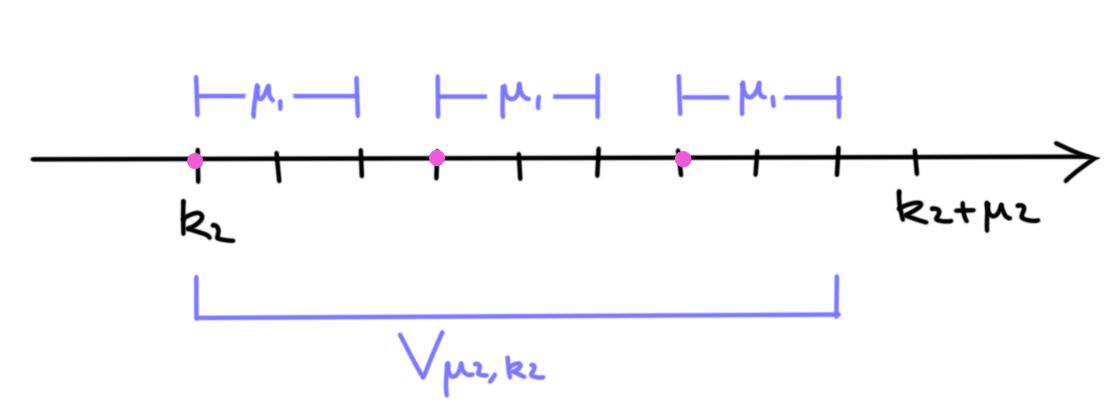
\includegraphics[scale=0.8]{9Junio_1}
\end{figure}


\QEDB
\end{itemize}
\end{dem}


\begin{comment}
3.- GLobal, una resolución
\phi: desfase
\mu: anchura
Teselado: A_{\pi, \mu}
Espacios periferia X_{\phi, \mu}

\end{comment}


\section{Análisis global: dos resoluciones}
Estamos listos para definir las versiones globales 
de los
espacios periferia locales
(c.f. definición \ref{definición de espacio M a g})
y bifocales locales
(c.f. definición \ref{espacios N_{a,g}});
para estos
últimos, vamos a usar 
un desfase $\phi$ y
una calibración $g=(z,s)$;
tendremos entonces que
considerar entonces a los teselados
$\cali{A}_{\phi, p}$ y $\cali{A}_{\phi, z}$.

En base a la contención establecida en el punto 4 
del teorema \ref{teo:hechos espacios periferia}
establecemos la siguiente definición.
\begin{defi}
\label{def: espacios Y}
Sean $\phi \in \IZ$ y $\mu_{1}, \mu_{2} \in \IN$, con $\mu_{1} | \mu_{2} $;
digamos que, $\mu_{1}a = \mu_{2}$. Sea la calibración
$g=(\mu_{1}, a)$.
Por $\La_{\phi,(\mu_{1}, a)}$ o por $\La_{\phi, g}$ 
denotaremos al espacio de las señales de $X_{\phi, \mu_{1}}$ que
son ortogonales a todas las de $X_{\phi, \mu_{2}}$, es decir,
\[
\La_{\phi, g} := X_{\phi , \mu_{1}} \cap  X_{\phi, \mu_{2}}^{\perp},
\]
o sea,
\[
\La_{\phi, g} = X_{\phi, \mu_{1}} \boxminus  X_{\phi, \mu_{2}}.
\]
Llamaremos a este el \textbf{espacio bifocal} respecto al punto
de anclaje $\phi$ y calibración $g$.
\end{defi}

\begin{ej}
Sean  $\mu_{1}=3$, $\mu_{2}=6$, $\phi=0$. La señal $x$ cuya gráfica 
se ilustra es elemento de $Y_{0,g}$.
\begin{figure}[H]
	\centering
	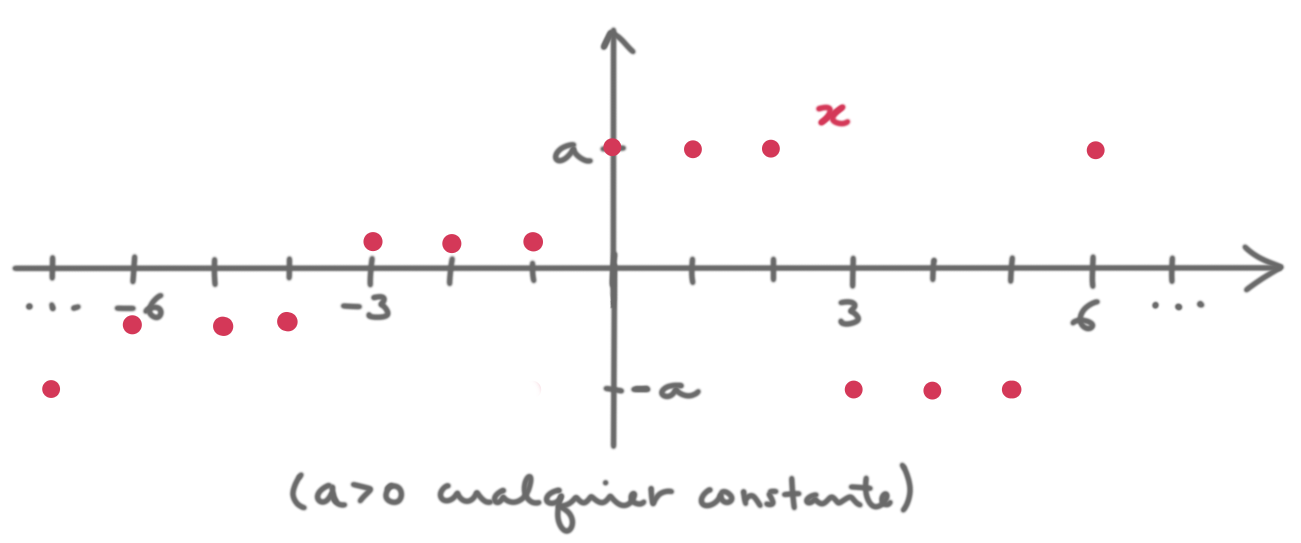
\includegraphics[scale=0.8]{2Junio_2}
\end{figure}
\end{ej}

Usando el que los espacios bifocales se
definen en términos de los espacios periferia
es sencillo establecer un lema análogo al
\ref{teo:hechos espacios periferia}.
\begin{lema} \label{lema: algunos hechos sobre espacios bifocales}
Sean $\phi, \phi_{1}, \phi_{2} \in \IZ$, $\mu_{1}, \mu_{2} \in \IN$
con $\mu_{1} | \mu_{2}$. Digamos que $\mu_{1}a = \mu_{2}$.
\begin{itemize}
\item $\Lambda_{\phi, (\mu_{1}, a)} = \{ 0\}$ si y sólo si
$a=1$, o sea, si y sólo si $\mu_{1}=\mu_{2}$.
\item Si $\mu_{1}=1$ y $\mu_{2}>1$, entonces 
$\Lambda_{\phi, (1 , a)}= X_{\phi, \mu_{2}}^{\perp}$.
\item Si $\phi_{1} \equiv \phi_{2} (mod \hspace{0.2cm} \mu_{2})$,
entonces 
$\Lambda_{\phi_{1}, (\mu_{1}, a)}= \Lambda_{\phi_{2}, (\mu_{1}, a)}$.
\end{itemize}
\end{lema}
\begin{dem}$\\ $
\TODO{cambiar tercer punto.}
\begin{itemize}
\item Por definición,
\begin{equation} \label{eq1: 20Oct}
\Lambda_{\phi, (\mu_{1}, a)}= X_{\phi, \mu_{1}} \cap
X_{\phi, \mu_{2}}^{\perp}.
\end{equation}

Si $\mu_{1}=\mu_{2}$, entonces 
$\Lambda_{\phi, (\mu_{1}, a)}$ es igual a la
intersección de un espacio con su complemento
ortogonal, luego, es igual al espacio $\{ 0 \}$;
recíprocamente, mostremos que si $\mu_{1} \neq \mu_{2}$
(o sea, que si $\mu_{1}< \mu_{2}$), entonces
siempre podemos encotrar un elemento no cero
en $X_{\phi, \mu_{1}}$ que es ortogonal a todo 
elemento de $X_{\phi, \mu_{2}}$. Digamos que
$\mu_{1} a = \mu_{2}$.


\begin{figure}[H]
	\centering
	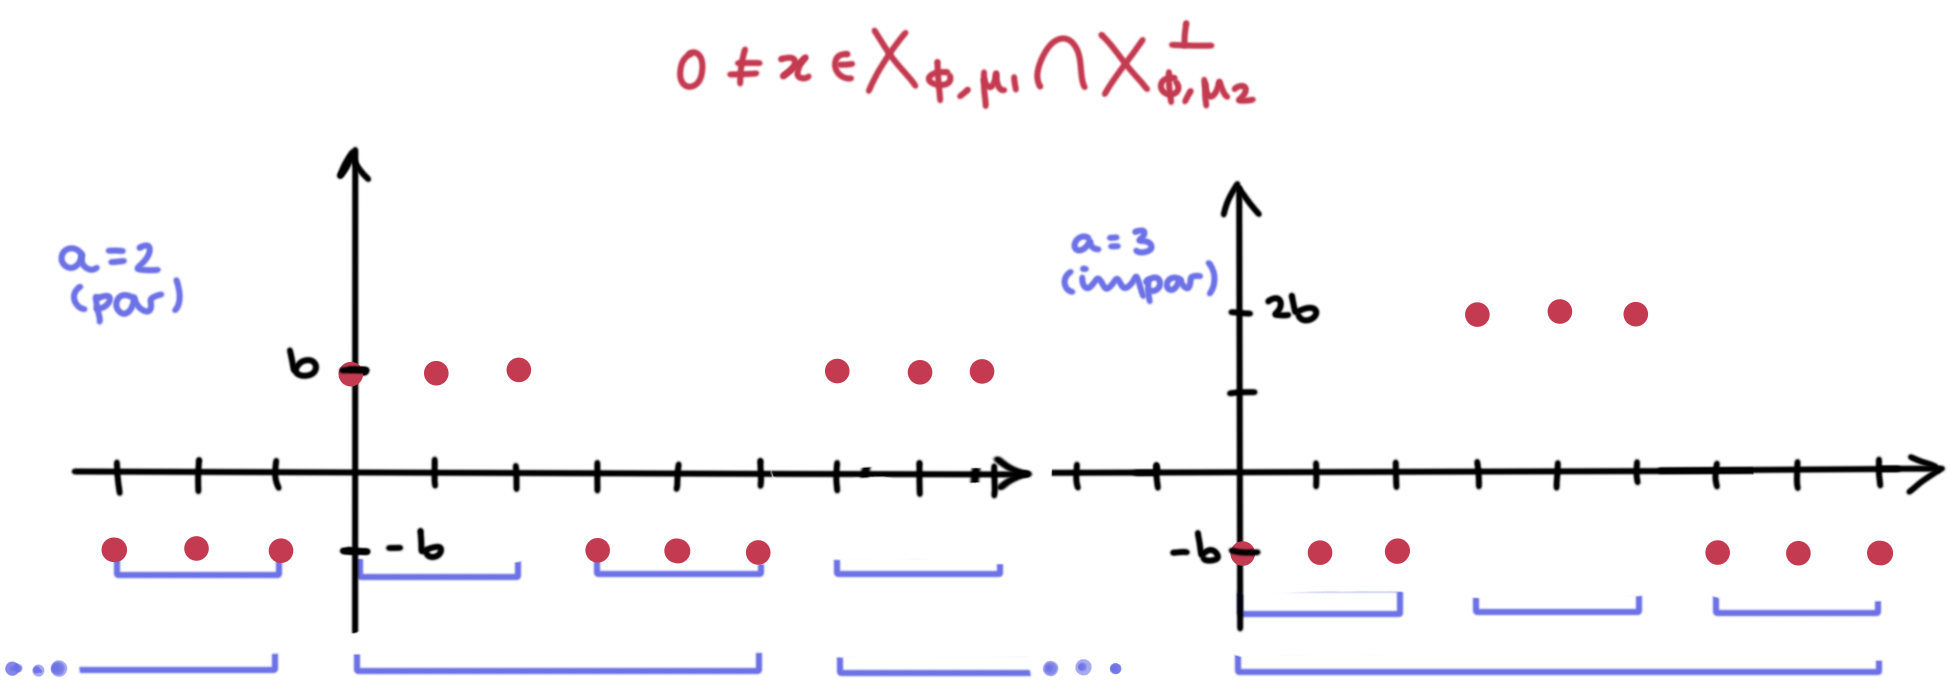
\includegraphics[scale=1]{20Oct_1}
	\caption{El argumento se basa en la paridad de $a$ y el 
	hecho de que sea mayor a uno.}
\end{figure}


\item Esto es claro pues, según
el primer punto del lema
\ref{teo:hechos espacios periferia},
$X_{\phi , 1}$ es todo el espacio $\ell^{2}(\IZ)$;
sustituyendo esto en \eqref{eq1: 20Oct}
llegamos a que
$\Lambda_{\phi, (1 , a)}= X_{\phi, \mu_{2}}^{\perp}$.

\item Según el segundo punto del lema
\ref{teo:hechos espacios periferia}, 
la hipótesis de congruencia de los puntos
de anclaje implica que 
$X_{\phi_{1}, \mu_{2}}=X_{\phi_{2}, \mu_{2}}$.
Puesto que $\mu_{1}$ divide a $\mu_{2}$,
también tenemos la congruencia
$\phi_{1} \equiv \phi_{2} (mod \hspace{0.2cm} \mu_{1})$,
luego, $X_{\phi_{1}, \mu_{1}}=X_{\phi_{2}, \mu_{1}}$;
así, 
\[
\Lambda_{\phi_{1}, (\mu_{1}, a)}=
X_{\phi_{1}, \mu_{1}} \cap X_{\phi_{1}, \mu_{2}}^{\perp}
=X_{\phi_{2}, \mu_{1}} \cap X_{\phi_{2}, \mu_{2}}^{\perp}
=\Lambda_{\phi_{2}, (\mu_{1}, a)}.
\]
\end{itemize}
$\QEDB$
\end{dem}

\begin{prop} \label{prop: ortogonalidad de espacios Y} 
Sean $\phi \in \IZ$, $\mu_{1}, \mu_{2}, \eta_{1}, \eta_{2} \in \IN$
con $\mu_{1} | \mu_{2}$, $\eta_{1} | \eta_{2}$,
$g_{\mu}=(\mu_{1}, \mu_{2})$,
$g_{\eta}=(\eta_{1}, \eta_{2})$. \\
Si $\mu_{2} | \eta_{1}$, entonces los espacios 
\[
\La_{\phi, g_{\mu}}, \hspace{0.2cm} \text{y} \hspace{0.2cm}
\La_{\phi, g_{\eta}}
\]
son ortogonales entre sí.
\end{prop}
\begin{dem} 
Por el punto 5 del lema
\ref{teo:hechos espacios periferia}, tenemos la
contención $X_{\phi, \eta_{1}} \subseteq X_{\phi, \mu_{2}}$,
por lo que 
$X_{\phi, \mu_{2}}^{\perp} \subseteq X_{\phi, \eta_{1}}^{\perp}$;
así,
\begin{align*}
\Lambda_{\phi, (\mu_{1}, s_{1})} = & 
X_{\phi, \mu_{1}} \cap X_{\phi, \mu_{2}}^{\perp} \\
\subseteq &  X_{\phi, \mu_{2}}^{\perp} \\
\subseteq &  X_{\phi, \eta_{1}}^{\perp} \\
\subseteq &  \Lambda_{\phi, (\eta_{1}, s_{2})}^{\perp},
\end{align*}
donde la última contención se da porque
$\Lambda_{\phi, (\eta_{1}, s_{2})} \subseteq X_{\phi, \eta_{1}}$.
\QEDB
\end{dem}



La siguiente proposición se encarga de proporcionar
bases para espacios bifocales.

\begin{teo} 
\label{teo:BON para Y z,p,l}
Dados un desfase $\phi$ y una calibración $g=(z,s)$, el conjunto

\begin{equation}\label{BON Lambda g,l-1}
\{ \lambda^{g,d}_{\phi+qp} : 0<d<s, \hspace{0.2cm} q \in \IZ  \}
\end{equation}
es una BON numerable del espacio $\Lambda_{\phi,g}$.
\end{teo}
\begin{dem} 
Consideremos a las particiones de $\IZ$
\begin{center}
$\cali{A}_{\phi, p}$= \{
$W_{q}:=  \alpha_{\phi+qp, p}$ : $ q \in \IZ$ \}
y $\cali{A}_{\phi, z}$.
\end{center}
Por definición,
\[
 \Lambda_{\phi, g}= X_{\phi, z} \cap X_{\phi, p}^{\perp},
\]
o sea, $\Lambda_{\phi, g}$
consta de las señales que
\begin{enumerate}
\item son constante en los alféizares de la colección $\cali{A}_{\phi, z}$ y
\item son ortogonales
a cualquier señal que sea constante en 
los alféizares de la colección $\cali{A}_{\phi, p}$.
\end{enumerate}

Mostremos primero que el conjunto propuesto
\eqref{BON Lambda g,l-1} es un subconjunto de $\Lambda_{\phi, g}$;
sea $\lambda^{g,d}_{\phi+qp}$ un elemento arbitrario de este.
Según la definición de esta señal (\TODO{¿aquí referencia?}),
su soporte está contenido
en el aféizar $W_{q}$ y
es constante en todos los elementos
de $\cali{A}_{\phi, z}$ ; por esto primero, si 
$x \in X_{\phi, p} $ arbitrario, 
\begin{equation}
\label{eq1: 26Sept}
< \lambda^{g,d}_{\phi+qp} , x > = 
< \lambda^{g,d}_{\phi+qp} , y_{q} >,
\end{equation}
donde $y_{q}:= x_{|\phi+qp, p}$. 
Según la proposición
\ref{prop: ventanas son constantes a la primera de Haar-Legendre}
existe $c$ escalar tal 
que $y_{q}=c \lambda_{\phi+qp}^{g,0}$; usando
esta expresión y la
ortogonalidad establecida en la proposición
\ref{prop: BON de M a g dual a la de Legendre discreta de Rs}, tenemos que
\begin{equation}
\label{eq2: 26Sept}
< \lambda^{g,d}_{\phi+qp} , y_{q} >=
< \lambda^{g,d}_{\phi+qp} , c \lambda_{\phi+qp}^{g,0}>
= c < \lambda^{g,d}_{\phi+qp} , \lambda^{g,0}_{\phi+qp} >=0;
\end{equation}
comparando \eqref{eq1: 26Sept} y \eqref{eq2: 26Sept},
se tiene que

\begin{equation*}
< \lambda^{g,d}_{\phi+qp} , x > = 0.
\end{equation*}
Con esto comprobamos que $\lambda^{g,d}_{\phi+qp} $
es ortogonal a todo elemento del espacio $X_{\phi, p}$, luego, 
su pertenencia al conjunto \eqref{BON Lambda g,l-1}.



Veamos ahora que \eqref{BON Lambda g,l-1} 
es un conjunto ortonormal.
Según la 
proposición \ref{prop: BON de M a g dual a la de Legendre discreta de Rs}, 
todos sus elementos son unitarios. Además,
si $\lambda^{g,d_{1}}_{\phi+q_{1}p}$ y
$\lambda^{g,d_{2}}_{\phi+q_{2}p}$ son dos elementos cualesquiera
de \eqref{BON Lambda g,l-1}, 
\begin{itemize}
\item si $q_{1} \neq q_{2}$, estas señales tendrán soportes
disjuntos (a saber, los alféizares $W_{q_{1}}$ y $W_{q_{2}}$)
y por lo tanto son ortogonales;
\item en caso contrario, por la 
proposición \eqref{BON Lambda g,l-1} podemos concluir
también la ortogonalidad.
\end{itemize}
Ya hemos probado entonces que \eqref{BON Lambda g,l-1}
es un subconjunto ortonormal de $\Lambda_{\phi, z, p}$. 
El que sea numerable es claro por su definición;
para terminar, mostremos que todo $x \in \Lambda_{\phi, z, p}$
es punto de cerradura del span de \eqref{BON Lambda g,l-1}. 

Lo que haremos será considerar a la descomposición de $x$
en las ventanas
\[
y_{q}:=x_{|\phi+qp, p}, \hspace{0.5cm} q \in \IZ,
\]
cuyos soportes son los
elementos de la partición $\cali{A}_{\phi ,p}$, y usar 
a estas para aproximar a 
la señal $x$ con combinaciones lineales
finitas de elementos de \eqref{BON Lambda g,l-1}. \\

Por estar contenido el soporte de la ventana $y_{q}$
en el alféizar $W_{q}:=\alpha_{\phi + qp}$ y
según el punto 1 de la lista del inicio, para toda $q$
se tiene la relación de pertenencia
$y_{q} \in \Lambda^{g}_{\phi+qp}$,
luego, por la proposición \ref{prop: BON de M a g},
\[
y_{q} \in span\{ \lambda^{g,d}_{\phi+qp} : 0\leq  d<s \}.
\]
Observe sin embargo que las señales
$y_{q}$ y $\lambda^{g,0}_{\phi+qp}$ son ortogonales (de
lo contrario, llegaríamos a la contradicción de que
$x \in X_{\phi, z}$ no es 
ortogonal a la señal $\lambda_{\phi+qp}^{g,0} \in X_{\phi, p}$,
pues
$
\langle x , \lambda_{\phi+qp}^{g,0}  \rangle
= \langle y_{q} , \lambda_{\phi+qp}^{g,0}  \rangle \neq 0
$), entonces,

\begin{equation}
\label{eq3: 26Sept}
y_{q} \in span\{ \lambda^{g,d}_{\phi+qp} : 0 < d < s \}. 
\end{equation}


Ahora sí; sea $\epsilon > 0$ cualquiera. \\
Como $\suma{z \in \IZ}{}{|x(z)|^{2}}< + \infty$,
es posible hallar una colección finita de alféizares
$W_{q_{i}}$, $1 \leq i \leq n$,
tal que

\[ || x-y || =
\suma{z \not\in \union{
i=1}{n}{W_{q_{i}}}}{}{|x(z)|^{2}} < \epsilon,
\]
donde $y:=\suma{i=1}{n}{y_{q_{i}}}$ 
es elemento del span de \eqref{BON Lambda g,l-1} pues,
gracias a \eqref{eq3: 26Sept},
cada $y_{q_{i}}$ puede expresarse como combinación lineal
finita de elementos de \eqref{BON Lambda g,l-1}.
\QEDB
\end{dem}

Establezcamos ahora relaciones entre los subespacios
de $\ell^{2}(\IZ)$ que hemos definido
hasta ahora.

\begin{prop}
(\textbf{Relación entre espacios periferia y espacios periferia locales})
Dada una calibración $g=(z,s)$, para todo 
desfase $\phi \in [0, z[ \cap \IZ$ se tiene que  
\[
X_{\phi, z}= \ameboxplus_{q \in \IZ} M_{\phi +qp,g}.
\]
\end{prop}
\begin{dem}
Por comodidad, fijemos un orden $\sigma : \IN \longrightarrow \IZ$,
$\sigma(j)=q_{j}$.
Necesitaremos considerar a los teselados
\[
\cali{A}_{\phi, z},
\hspace{0.2cm} \text{y} \hspace{0.2cm}
\cali{A}_{\phi, p}=\{ \alpha_{\phi+qp, p} : \hspace{0.2cm} q \in \IZ\}.
\]


\begin{itemize}
\item[$\subseteq$)]
Sea $x \in X_{\phi,z}$. 
Sea la descomposición de $x$ en ventanas con soportes
los elementos de $\cali{A}_{\phi,p}$ (c.f.
proposición \ref{prop: descomposicion de una señal en ventanas});
\begin{equation}
\label{eq1: 15Nov}
x=\suma{j =1}{\infty}{y_{q_{j}}}, \hspace{0.2cm}
\text{con} \hspace{0.2cm} y_{q_{j}}=x_{|\phi + q_{j}p, p};
\end{equation}


observe que, al igual que $x$, las ventanas
$y_{q_{j}}$ son todas constantes en los elementos
de $\cali{A}_{\phi, z}$, pero además
la señal
$y_{q_{j}}$ es cero fuera del
alféizar $\alpha_{\phi+qp, p}$, luego,
según la observación \ref{prop: BON1 de Lambda g, k},
$y_{q_{j}} \in M_{\phi+q_{j}p, g}$.

Sea $\epsilon >0$; según
\eqref{eq1: 15Nov}, es posible encontrar $n \in \IN$
tal que
\[
|| x - y || =
||\suma{\substack{ {q \neq q_{i}}, \\  {1 \leq i \leq n} }}{}{y_{q}}||< 
\epsilon,
\]
donde 
$y:= \suma{i=1}{n}{y_{q_{i}}}$
es, según lo notado antes, elemento de la suma
$\suma{i=1}{n}{M_{\phi+q_{i}p, g}}$, por lo tanto, elemento 
del espacio $\union{n \in \IN}{}{\suma{j=1}{n}{M_{\phi+q_{n}p, g}}}$.
Como $\epsilon >0$ fue arbitrario, tenemos que
\[
x \in \overline{\union{n \in \IN}{}{\suma{j=1}{n}{M_{\phi+q_{n}p, g}}}},
\]
o sea,  
según la proposición
\ref{prop: caracterizacion suma infinita de subespacios ortogonales},
que 
$x \in \ameboxplus_{q \in \IZ} M_{\phi +qp,g}.$

\item[$\supseteq$ )] 
Según las caracterizaciones dadas en 
la observación 
\ref{prop: BON1 de Lambda g, k}
y en el teorema
\ref{teo:caracterizacion espacios periferia}, 
claro que
para toda $q \in \IZ$ se tiene la contención
\[
M_{\phi + q p, g} \subseteq X_{\phi, z},
\]
por lo tanto, la contención
\begin{equation}
\label{eq1: 14Nov}
\union{n \in \IN}{}{\suma{j=1}{n}{M_{\phi+q_{n}p, g}}}
\subseteq X_{\phi, z};
\end{equation}
como $X_{\phi, z}$ es, por definición, un subespacio
cerrado de $\ell^{2}(\IZ)$, de
\eqref{eq1: 14Nov} se deduce que
\[
\ameboxplus_{q \in \IZ} M_{\phi +qp,g}
=
\overline{\union{n \in \IN}{}{\suma{j=1}{n}{M_{\phi+q_{n}p, g}}}}
\subseteq X_{\phi, z}.
\]
$\QEDB$
\end{itemize}
\end{dem} 

La demostración de la siguiente proposición
es totalmente análoga a la anterior, por lo que se omite.
\begin{prop}
(\textbf{Relación entre espacios bifocales y espacios
bifocales locales.})
Dada una calibración $g=(z,s)$, para todo 
desfase $\phi \in [0, z[ \cap \IZ$ se tiene que  
\[
\Lambda_{\phi, g}= \ameboxplus_{q \in \IZ} N_{\phi +qp,g}.
\]
\end{prop}


\begin{prop} (\textbf{Relación entre espacios periferia y espacios 
bifocales})
\label{prop: relacion espacios periferia y espacios lambda}
Dados $\phi \in \IZ$ un desfase y
$g=(z,s)$ una calibración,
\[
X_{\phi ,z}= \Lambda_{\phi, g} \boxplus X_{\phi,p}.
\]
\end{prop}
\begin{dem}
Por definición,
\[
\Lambda_{\phi,g}= X_{\phi,z} \boxminus X_{\phi,p},
\]
luego, como el espacio periferia 
$X_{\phi,p}$ es cerrado y, según el teorema 
\ref{teo:hechos espacios periferia} está contenido en
el espacio $X_{\phi,z}$, podemos concluir, por la proposición
\ref{prop: pasar de resta ortogonal a suma ortogonal},
que en efecto $X_{\phi, z}$ es la suma ortogonal 
de $\Lambda_{\phi, z,p}$ con $X_{\phi, p}$. 
\QEDB
\end{dem}
\begin{comment} Esta demostración también
estaba bien, pero ya no es necesaria.
\begin{dem}
Por definición de $\Lambda^{g,l}$, todos los elementos
de este espacio son ortogonales a los de 
$X_{p,l}$; además, tanto $\Lambda^{g,l}$ como
$X_{p,l}$ están contenidos
en $X_{z,l}$, luego, por ser
este último cerrado bajo sumas (por ser subespacio
de $\ell^{2}(\IZ)$) tenemos
la contención $\Lambda^{g,l} + X_{p,l} \subseteq X_{z,l}$. 
Resta entonces demostrar que
también ocurre $$X_{z,l} \subseteq \Lambda^{g,l} + X_{p,l}.$$ 
Sea pues $x \in X_{z,l}$; según el teorema
\ref{teo:caracterizacion espacios periferia},
$x$ es constante en 
cada uno de los alféizares de la colección $\cali{A}_{2}$
y, si
\[
y_{q}=x_{|p, l+qp}
\]
es su ventana con soporte contenido en $W_{q}=V_{p, l+qp}$,
entonces $y_{q} \in \Lambda^{g}_{l+qp}$.
Las proposiciones \ref{prop: BON de M a g} y 
\ref{prop: BON1 de Lambda g, k} nos dan dos bases
ortonormales para este espacio; recordando la definiciones de
las señales de esta última base,
podemos establecer una ecuación de la forma
\[
 \suma{d=0}{s-1}{a_{q,d}\lambda^{g,d}_{l+qp}}
 = y_{q} =
  \suma{d=0}{s-1}{\sqrt{z}x(l+qp+dz)\chi_{z, l+qp+dz}};
\]
así, por la identidad de Parseval 
(inciso f) del teorema \ref{thm: Coway, 4.13}),
\[
\suma{d=0}{s-1}{|a_{q,d}|^{2}} = ||y_{q}||^{2}
= \suma{d=0}{s-1}{z|x(l+qp+dz)|^{2}}.
\]
Haciendo variar a $q$ en $\IZ$, tenemos por el lado
derecho de esta última igualdad que
\[
\suma{q \in \IZ}{}{||y_{q}||^{2}}
\leq \suma{q \in \IZ}{}{z|x(l+qp+dz)|^{2}}
= z \suma{\nu \in \IZ}{}{|x(l+\nu z)|^{2}} = z ||x||^{2}
< \infty.
\]


Ahora sí, propongamos unas señales
$a \in \Lambda^{g,l}$, $b \in X_{p,l}$ tales que $x=a+b$. \\
Sean 

\[
a := \suma{q \in \IZ}{}{\left(\suma{d=1}{s-1}{a_{q,d}\lambda_{l+qp}^{g,d}} \right)},
\hspace{0.5cm}
b:= \suma{q \in \IZ}{}{a_{q,0}\lambda_{l+qp}^{g,0}}.
\]
El que estas en efecto sean señales
(i.e. elementos de $\ell^{2}(\IZ)$) 
se deduce directamente
de la convergencia establecida antes; por ejemplo,

\begin{align*}
|| \suma{i=1}{n}{\left(\suma{d=1}{s-1}{a_{q_{i},d}\lambda_{l+q_{i}p}^{g,d}} \right)} ||^{2} & = \suma{i=1}{n}{|| \suma{d=1}{s-1}{a_{q_{i},d}\lambda_{l+q_{i}p}^{g,d}} ||^{2}} \\
& = \suma{i=1}{n}{  \suma{d=1}{s-1}{|| a_{q_{i},d} ||^{2}} } \\
& \leq \suma{i=1}{n}{  \suma{d=0}{s-1}{|| a_{q_{i},d} ||^{2}} } 
= \suma{i=1}{n}{|| y_{q_{i}} ||^{2}},
\end{align*}
\noindent 
dándose las primeras dos igualdades
por la ortogonalidad de las señales involucradas.

Puesto que la suma de los límites de dos series convergentes 
es igual al límite de su suma,
y por el resultado establecido en la proposición
\ref{prop: descomposicion de una señal en ventanas},
tenemos que
\[
\suma{q \in \IZ}{}{\left(\suma{d=1}{s-1}{a_{q,d}\lambda_{l+qp}^{g,d}} \right)}+
\suma{q \in \IZ}{}{a_{q,0}\lambda_{l+qp}^{g,0}}
= \suma{q \in \IZ}{}{\left(\suma{d=0}{s-1}{a_{q,d}\lambda_{l+qp}^{g,d}} \right)}
= \suma{q \in \IZ }{}{y_{q}} = x;
\]
\noindent 
observe que el primer sumando, según el teorema
\ref{teo:BON para Y z,p,l}, es elemento 
de $\Lambda^{g,l}$; el segundo sumando es una 
señal constante en cada alféizar de la partición 
$\cali{A}_{1}$, por lo tanto, según el
teorema \ref{teo:caracterizacion espacios periferia},
elemento de $X_{p,l}$. 
\QEDB
\end{dem}
\end{comment}

\begin{notacion}
\label{notacion: calibracion g j}
Cuando se tenga una calibración $g=(z,s)$, 
para cada $j \in \IN$ definimos la calibración
\[
g_{j}:=(s^{j}z, s).
\]
\end{notacion}

Dada una calibración $g=(z,s)$ 
y un punto de anclaje $\phi$,
según la proposición 
\ref{prop: relacion espacios periferia y espacios lambda}, todo elemento
del espacio periferia $X_{z, \phi}$ puede expresarse
de forma única como la suma de 
\begin{itemize}
\item un elemento del espacio periferia $X_{\phi,z}$ 
que sea ortogonal a todo elemento de $X_{\phi,p}=X_{\phi, zs}$ con
\item un elemento de $X_{\phi, p}=X_{\phi, zs}$.
\end{itemize}

Podemos repetir este argumento, esta vez pensando en
los espacios periferia $X_{\phi, p}=X_{\phi, zs}$ y $X_{\phi, zs^{2}}$,
y deducir la siguiente cadena de igualdades:


\begin{align*} \label{eq7: 16Agosto}
X_{\phi, z} & = \Lambda_{\phi,g} \boxplus X_{\phi,p} \\
& = \Lambda_{\phi, g_{0}} \boxplus X_{\phi,sz} \\
& = \Lambda_{\phi, g_{0}} \boxplus (\Lambda_{\phi, g_{1}}
\boxplus X_{\phi, s^{2}z}) \\ 
& = (\Lambda_{\phi, g_{0}} \boxplus \Lambda_{\phi, g_{1}})
\boxplus X_{\phi, s^{2}z}. 
\end{align*}
Este razonamiento
se generaliza fácilmente
para un $J \in \IN$ cualquiera,
logrando expresar al
espacio periferia $X_{\phi,z}$
como suma de $J+2$ subespacios de $\ell^{2}(\IZ)$
ortogonales dos a dos.

\begin{obs} 
Fijados 
un desfase $\phi \in \IZ$ y
una calibración
$g=(z,s)$,
si $J \in \IN$, entonces
\begin{equation} 
\label{eq: espacio periferia como suma ortonormal de J+1 espacios}
X_{\phi, z}= \left( \ameboxplus_{j=0}^{J}\La_{\phi, s^{j}z, s^{j+1}z} \right) \boxplus
X_{\phi, s^{J+1}z}.
\end{equation}
\end{obs}

\begin{figure}[H]
	\centering
	\includegraphics[scale=0.5]{28Junio_1}
	\caption{\TODO{Cambiar notación} Así como agrupamos $s$ alféizares contiguos de tamaño $z$ para formar alféizares de tamaño p (construyendo así, a partir de los elementos de la partición 
$\cali{A}_{\phi, z}$ a los de la partición 
$\cali{A}_{\phi, p}=\cali{A}_{\phi, sz}$), 
podemos agrupar $s$ de estos alféizares
contiguos para formar unos de tamaño $sp$ 
(construyendo así, a partir de los elementos de la partición 
$\cali{A}_{\phi, sz}$ a los de la partición 
$\cali{A}_{\phi, s^{2}z}$), y así sucesivamente. 
Fijado un $j \in \IN$,
según la ecuación
\ref{eq: espacio periferia como suma ortonormal de J+1 espacios}, 
podremos expresar a una señal cualquiera de $X_{z,l}$ 
(que es una señal que es constante en todos los elementos de 
$\cali{A}_{\phi, z}$) 
de forma única como la suma de una señal 
constante en todo elemento de $\cali{A}_{\phi, s^{J+1}z}$
con señales constantes en los elementos de $\cali{A}_{\phi, s^{j}z}$ y ortogonales a todas las que sean constantes en los elementos de $\cali{A}_{\phi, s^{j+1}}$ ($0 \leq j \leq J$).}
\end{figure}


\begin{teo} 
\label{teo: paso al limite, suma ortogonal}
(paso al límite de 
la igualdad
\eqref{eq: espacio periferia como suma ortonormal de J+1 espacios})
Dados un desfase $\phi$ y una calibración $g=(z,s)$,
\[
X_{\phi,z} = \ameboxplus_{j = 0}^{\infty} \La_{\phi, g_{j}}.
\]
\end{teo}
\demostracion
Observe primero que, para toda $j$,
\begin{equation} \label{ec2: 16 Agosto}
\La_{\phi,g_{j}} = X_{\phi,s^{j}z} \cap
X^{\perp}_{\phi,s^{j+1}z} \subseteq X_{\phi,s^{j}z} \subseteq X_{\phi,z},
\end{equation}
\noindent
siendo cierta la última contención por el punto 4 del teorema 
\ref{teo:hechos espacios periferia}.\\
Ahora bien, si 
$x \in \ameboxplus_{j = 0}^{\infty} \La_{\phi,g_{j}}$,
según la caracterización dada en la proposición
\ref{prop: caracterizacion suma infinita de subespacios ortogonales},

\begin{equation} \label{ec1: 16 Agosto}
x = \limite{n \rightarrow \infty }{\suma{j=0}{n}{x_{j}}}
\end{equation}
para unos únicos
$x_{j} \in \La_{\phi,g_{j}}$.
Según la última contención de 
\eqref{ec2: 16 Agosto}, cada
señal $\suma{j=0}{n}{x_{j}}$ es elemento del 
subsepacio cerrado $X_{\phi,z}$ de $\ell^{2}(\IZ)$;
así, \eqref{ec1: 16 Agosto} expone a $x$ como punto 
de cerradura del espacio $X_{\phi,z}$, o sea, como elemento de este.\\

Demostremos ahora la otra contención; sea
$x \in X_{\phi,z}$. Sea 
$\epsilon >0$.
Puesto que $x$ es elemento de $\ell^{2}$, las colas
de la serie $\suma{q \in \IZ}{}{x(q)}$ tienden a cero;
esto nos permite considerar una ventana $\hat{x}$ de $x$
tal que $||x- \hat{x} ||$ sea una cola de la serie menor
a $\frac{\epsilon}{2}$, o sea, una ventana tal que
\[
||x- \hat{x} || < \frac{\epsilon}{2}
\]
y que, sin pérdida de generalidad,pertenezca,
al igual que $x$, al espacio
periferia $X_{\phi,z}$.
\footnote{informalmente hablando, ``cortamos a
la señal $x$ en un lugar adecuado para que la ventana resultante
sea también constante en los elementos de la partición $\cali{A}_{\phi,z}$''
y, además, se encuentre a una distancia de $x$ menor a $\frac{\epsilon}{2}$.}

Si $J$ es un número natural,
podemos usar la igualdad
\eqref{eq: espacio periferia como suma ortonormal de J+1 espacios} 
para expresar a $\hat{x}$ como
\[
\hat{x} = \hat{w}_{J} + \hat{x}_{J},
\]
donde
\begin{itemize}
\item $\hat{w}_{J}$ es combinación lineal (finita) de elementos 
de la familia 
ortogonal dos a dos $\La:=(\La_{\phi, g_{j}})_{j=0}^{\infty}$, y
\item $\hat{x}_{J} = \Pi_{X_{\phi, s^{J+1}z}}(v) \in X_{\phi, s^{J+1}z}$ 
(c.f. proposición \ref{prop: elemento de la suma ortogonal de subespacios}).
\end{itemize}
Afirmamos que podemos encontrar $J$ lo suficientemente grande
como para que la norma de la proyección $ \hat{x}_{J} $ sea menor
a $\frac{\epsilon}{2}$; con esto podremos concluir que $\hat{w}_{J}$
está a una distancia de $x$ menor a $\epsilon$, pues, por
la desigualdad triangular,
\[
||x- \hat{w}_{J} || \leq  ||x- \hat{x} || + || \hat{x} - \hat{w}_{J} ||
=  ||x- \hat{x} || + || \hat{x}_{J}|| < \frac{\epsilon}{2} + \frac{\epsilon}{2} 
= \epsilon
\]
(como $\epsilon >0$ fue arbitrario, con esto podremos concluir,
como queríamos, que
$v$ es punto de cerradura de 
$\union{n \in \overline{\IN}}{}{\ameboxplus_{j=0}^{n} \La_{\phi,g_{j}}}$, o sea, elemento
del espacio $\ameboxplus_{j = 0}^{\infty} \La_{\phi,g_{j}}$). \\

La clave radica en observar que, por ser el soporte de la ventana 
$\hat{x}$
finito, para $J$ lo suficientemente grande este estará contenido
en a lo más dos elementos
\footnote{Como $s$ y $z$ son constantes mayores a uno, 
$\limite{J \rightarrow \infty}{s^{J+1}z}= \infty$,
luego, escogiendo $J$ lo suficientemente grande, podemos
asegurar que los elementos de la partición
$\cali{A}_{\phi,s^{J+1}z}$ tienen anchuras tan grandes como queramos.}
de la partición  $\cali{A}_{\phi,s^{J+1}z}$
(dependiendo de si el desfase $\phi$ esté o no entre
dos puntos contenidos en el soporte),
a saber, en $\alpha_{\phi,s^{J+1}z}$ y en $\alpha_{\phi-s^{J+1}z, s^{J+1}z}$;
es decir,

\[
sop(\hat{x}) \subseteq \alpha_{\phi,s^{J+1}z} \cup 
\alpha_{\phi-s^{J+1}z, s^{J+1}z}.
\]
Por ser $sop(\hat{x})$ un conjunto finito de $\IZ$, podemos considerar
a su máximo y su mínimo, que denotamos por $A$ y $B$, respectivamente;
tomando a $J$ lo suficientemente grande, podemos suponer que
\[
A \in \alpha_{\phi,s^{J+1}z} \hspace{0.2cm} \text{y}
\hspace{0.2cm} B \in \alpha_{\phi-s^{J+1}z, s^{J+1}z}.
\]

\begin{figure}[H]
	\centering
	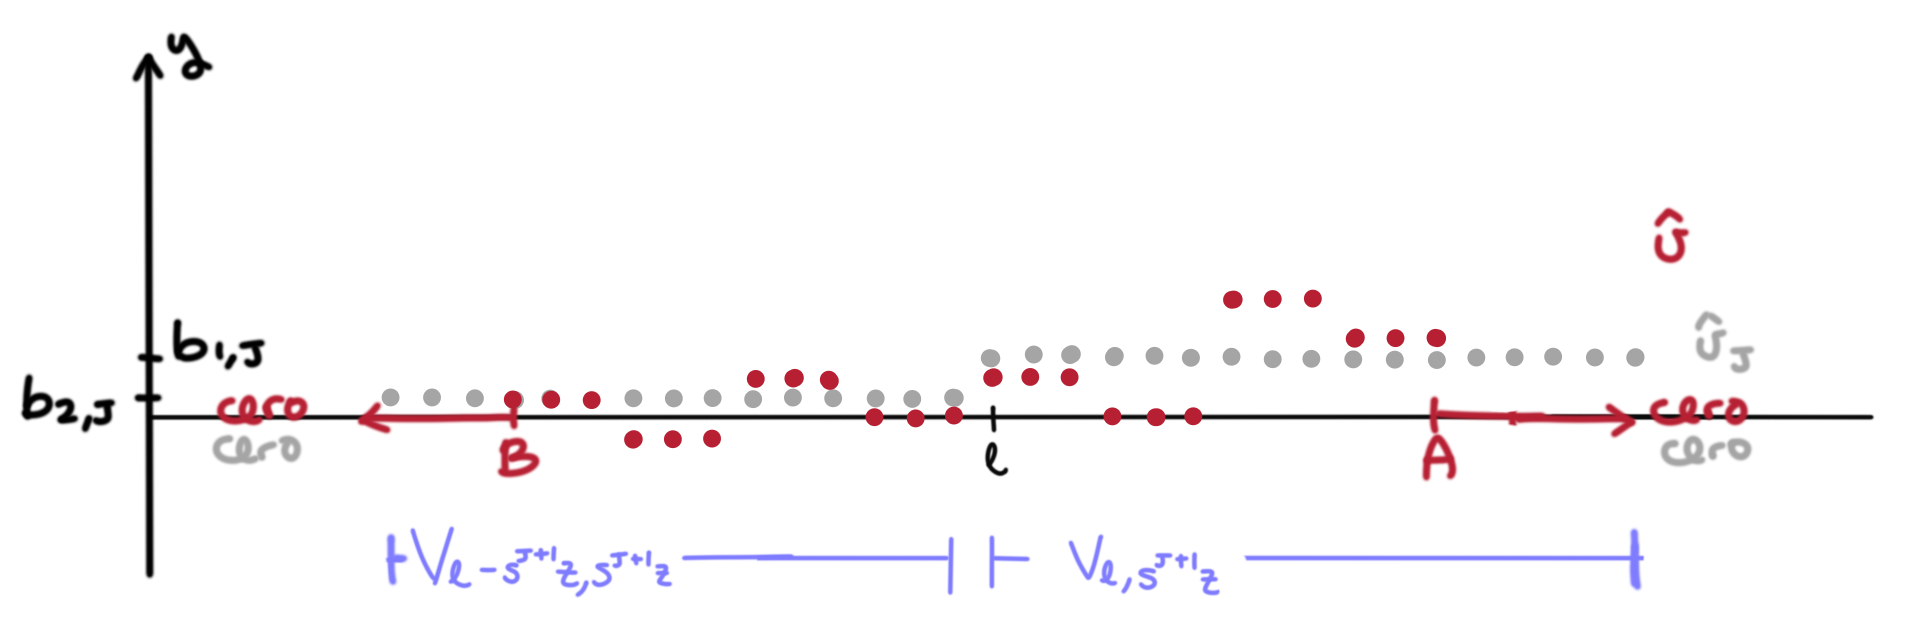
\includegraphics[scale=0.8]{13Julio_1}
	\caption{\TODO{Cambiar notación.}}
\end{figure}


Digamos que en $\alpha_{\phi,s^{J+1}z}$ y 
$\alpha_{\phi-s^{J+1}z, s^{J+1}z}$ la señal $\hat{x}_{J}$ toma los valores
$b_{1,J}$ y $b_{2,J}$,
respectivamente; puesto que $\hat{x}$ vale cero en los
demás elementos de $\cali{A}_{\phi, s^{J+1}}$ y 
$\hat{x}_{J}$ es el elemento
del espacio $ X_{\phi, s^{J+1}z}$
que mejor aproxima a $\hat{x}$ (pues, como dijimos
arriba, $\hat{x}_{J}$ es la proyección
de $\hat{x}$ al espacio periferia $X_{\phi,s^{J+1}z}$), 
claro que esta señal
también vale cero en los alféizares distintos a 
$alpha_{\phi,s^{J+1}z}$ y $V\alpha_{\phi-s^{J+1}z, s^{J+1}z}$,
luego, su norma simplemente es
\begin{equation} \label{eq 0: 22Agosto}
|| \hat{x}_{J} || = \sqrt{s^{J+1}z} \cdot \sqrt{b_{1, J}^{2} + b_{2, J}^{2}}.
\end{equation}

\noindent
Observe que
$b_{1,J}$ y $b_{2,J}$ son las elecciones de $x$ y $y$
que minimizan a la función de dos variables

\[
f(x,y)= \sqrt{z} \sqrt{\suma{i=l}{A}{(x(i)-x)^{2}}+(s^{J+1}z-A)x^{2}}+
\sqrt{z} \sqrt{\suma{i=B}{l-1}{(x(i)-y)^{2}}+(s^{J+1}z-B)y^{2}};
\]
\noindent
equivalentemente, $b_{1,J}$ es el mínimo de la 
función real
\[
g(x)=\sqrt{z} \sqrt{\suma{i=l}{A}{(x(i)-x)^{2}}+(s^{J+1}z-A)x^{2}}
\]
y $b_{2,J}$ el mínimo de la función real
\[
h(y)=\sqrt{z} \sqrt{\suma{i=B}{l-1}{(x(i)-y)^{2}}+(s^{J+1}z-B)y^{2}}.
\]
\noindent
Derivando estas expresiones e igualando a cero,
llegamos a que
\begin{equation} \label{eq 1: 22Agosto}
b_{1,J}= \frac{cte_{1}}{s^{J+1}z} \hspace{0.4cm} \text{y}
\hspace{0.4cm} b_{2,J}= \frac{cte_{2}}{s^{J+1}z},
\end{equation}
donde $cte_{1}$ y $cte_{2}$ son las siguientes constantes:
\[
cte_{1}:= \suma{i=l}{A}{x(i)}, \hspace{0.4cm}
cte_{2}:= \suma{i=B}{l-1}{x(i)}.
\]
Sustituyendo \eqref{eq 1: 22Agosto}
en \eqref{eq 0: 22Agosto}, concluimos que
\[
|| \hat{x}_{J} || = \frac{\sqrt{cte_{1}^{2}+ cte_{2}^{2}}}{\sqrt{s^{J+1}z}}
\rightarrow 0 \hspace{0.5cm} \text{conforme} 
\hspace{0.2cm} J \rightarrow \infty.
\]
\QEDB



\section{Descomposición de señales respecto a los espacios bifocales}

Hasta el momento, hemos introducido
las nociones de un desfase $\phi$, una calibración $g=(z,s)$,
con $z$ el zoom/resolución, $s$ la escala y 
$p:=zs$ el ámbito (pensando a $z$ y a $p$
como anchuras de alféizares, jugando entonces $s$
el rol de \textbf{factor de cambio de escala} entre una anchura y otra).
En esta sección, vamos a dar una descomposición
de una señal cualquiera que, via ciertos pesos que
cumplan una condición de normalización, \textbf{considere
a todos los desfases y calibraciones posibles;}
los detalles de este desarrollo,
su significado y su importancia
se exponen a continuación.

\subsection{Sucesiones de pesos}

Primero, veamos cómo nos interesará formar sucesiones
de pesos que consideren a todas las 
posibles combinaciones de desfases, 
escalas y resoluciones posibles.

Fijemos una escala $s \geq 2$.
Si $z \in \IN$ es una anchura cualquiera,
como consecuencia
del teorema fundamental de la aritmética, existen únicos
\begin{center}
$j \in \overline{\IN}$ y $z_{0} \in \IN$ con $s \nmid z_{0}$
\end{center}
tales que 
\begin{equation}
\label{eq1: 12Oct}
z=s^{j}z_{0};
\end{equation}

\noindent
esto nos permite entonces definir a una biyección
$$\sigma_{s}: \IN \longrightarrow \overline{\IN} \times 
\{ z_{0} \in \IN : s \nmid z_{0} \} $$ como sigue:
\begin{equation}
\label{eq: definicion de la biyeccion sigma s}
\sigma_{s}(z)=(\sigma_{s,1}(z), \sigma_{s,2}(z))=(j,z_{0}),
\end{equation}
\noindent
donde $z$ es como en \eqref{eq1: 12Oct}

Fijar un $s$ es fijar el factor
de multiplicación que aceptamos para pasar de anchuras
de subalféizares a anchuras de alféizares; el considerar
la descomposición \eqref{eq1: 12Oct} de una anchura $z$
puede pensarse como el buscar 
de qué anchura inicial $z_{0}$
partir para, 
a partir de una calibración inicial $g=(z_{0},s)$,
después de una cantidad finita de ampliaciones
(con factor $s$), poder llegar
a una calibración $g_{j}= (z_{0}s^{j}, s)$
en base a la cual se construyen subalféizares
de tamaño $z_{0}s^{j}=z$.


Con la escala $s$ todavía fija, formamos el 
siguiente conjunto de índices:
\[
I_{s}= \{ (\phi, z_{0}, s) \in \IZ \times \IN \times \{s\}  : s \nmid z_{0} \}.
\]

Ahora consideramos al conjunto de índices
formado a partir de los $I_{s}$, donde $s$
es un entero mayor o igual a dos:

\begin{equation}
\label{eq10: 14Oct}
I= \union{s=2}{\infty}{I_{s}},
\end{equation}
siendo $I$ numerable por ser unión numerable de 
conjuntos numerables.

Si en base a este conjunto de índices $I$
consideramos una familia de pesos
\begin{equation}
\label{eq10: 29Sept}
\Omega=\{ \omega_{\phi, z_{0}, s} \in [0,1] : (\phi, z_{0}, s) \in I \}
\end{equation}
tal que
\begin{equation}
\label{eq11: 29Sept}
\suma{(\phi, z_{0}, s) \in I}{}{\omega_{(\phi, z_{0}, s)}}=1,
\end{equation}
podemos, en base a esta, descomponer a una señal
arbitraria $x \in \ell^{2}(\IZ)$ como se muestra
en el siguiente resultado.
\begin{prop} \label{prop: descomposicion de señal respecto a pesos}
Si $x=(x_{k})_{k \in \IZ}$ es un elemento de
$\ell^{2}(\IZ)$ y $\Omega$ es una familia de pesos como
en \eqref{eq10: 29Sept} que satisface
la condición \eqref{eq11: 29Sept}, entonces
\[
x= \suma{(\phi, z_{0}, s) \in I}{}{\omega_{\phi, z_{0}, s}x}.
\]
\end{prop}
\demostracion
Observe antes que, según \eqref{eq10: 29Sept}, la serie
$\suma{(\phi, z_{0}, s) \in I}{}{\omega_{\phi, z_{0}, s}}$
es de términos no negativos, luego,
la condición \eqref{eq11: 29Sept} significa que
converge absolutamente a uno, por lo que la convergencia
y el límite son invariantes bajo reordenaciones, y la
convergencia equivale a que, para todo $\epsilon>0$
sea posible encontrar un conjunto $A \subseteq I$
finito tal que
\[
|\left(\suma{(\phi, z_{0}, s) \in I-A}{}{\omega_{\phi, z_{0}, s} }-1 \right) |
< \epsilon;
\]
esto claramente nos permite acotar a la norma
\[
|| \suma{(\phi, z_{0}, s) \in A}{}{\omega_{\phi, z_{0}, s} x} -x||=
|| \left(\suma{(\phi, z_{0}, s) \in A}{}{\omega_{\phi, z_{0}, s} }-1 \right) x||
= |\left(\suma{(\phi, z_{0}, s) \in A}{}{\omega_{\phi, z_{0}, s} }-1 \right) |
\cdot ||x||,
\]
pues $||x||$ es una constante.
$\QEDB$
\subsection{Descomposición de señales}


Fijemos una familia
$\Omega$ de pesos como
en \eqref{eq10: 29Sept} que satisface
la condición \eqref{eq11: 29Sept}.
\noindent
Dados un punto de anclaje $\phi$ y una calibración
$g=(z_{0},s)$, podemos descomponer 
al espacio $\ell^{2}(\IZ)$
(usando la proposición
\ref{prop: relacion espacios periferia y espacios lambda}
y el 
teorema \ref{teo: paso al limite, suma ortogonal})
como suma de subespacios de 
este ortogonales dos a dos
como sigue:

\begin{align}
\ell^{2}(\IZ) = & X_{\phi, 1} \nonumber \\
= & 
\Lambda_{\phi, (1,z_{0})} \boxplus X_{\phi, z_{0}} \nonumber  \\
= & 
\Lambda_{\phi, (1,z_{0})} \boxplus \left( 
\ameboxplus_{j = 0}^{\infty} \La_{\phi, g_{j}} \right), 
\label{eq1: 14Oct} 
\end{align}
luego, si $x=(x_{k})_{k \in \IZ} \in \ell^{2}(\IZ)$
es una señal cualquiera, 
según la igualdad \eqref{eq1: 14Oct} y la 
proposición \ref{prop: caracterizacion suma infinita de subespacios ortogonales}, tenemos que
\begin{equation}
\label{eq: descomposicion de x dada una calibracion g}
x= \Pi_{\Lambda_{\phi, (1,z_{0})}}(x) + \suma{j=0}{\infty}{\Pi_{\La_{\phi,g_{j}}}(x) },
\end{equation}
donde la calibración $g_{j}$ se forma a partir
de la inicial $g$ como se especifica en 
\ref{notacion: calibracion g j}.
Es en base a esta expresión (que descompone a $x$ respecto 
a una elección de desfase $\phi$ y calibración $g=(z_{0},s)$
particular) y a la establecida en
la proposición 
\ref{prop: descomposicion de señal respecto a pesos}
de una señal en términos de pesos que consideren a \textbf{todos}
los valores posibles para los parámetros $\phi$, $z_{0}$
y $s$, que queremos descomponer a la señal $x$
y llegar a una expresión de esta 
en términos de
sus proyecciones en todos los
espacios bifocales; nuestro objetivo
es pues,
a partir de una familia de pesos
$\Omega$ como en
\eqref{eq10: 29Sept} que satisfaga
la relación \eqref{eq11: 29Sept},
construir una familia 
\[
\rho=\{ \rho_{\phi, (z,s)}: \hspace{0.1cm} z \geq 1, s \geq 2, 0 \leq
\phi \leq zs \}
\]
tal que una expresión de la forma
\footnote{Note que en \eqref{eq: descomposicion de x buscada}
se hace variar
primero a $s$ y $z$ (los parámetros necesarios para
dar las anchuras de alféizares
con los cuales partir 
a $\IZ$), y al final a $\phi_{0}$; la acotación
para este último parámetro, según el lema
\ref{lema: algunos hechos sobre espacios bifocales},
es razonable, pero, en los cálculos que siguen,
para poder considerar a todos los espacios 
bifocales posibles, 
\textit{a priori} \textbf{no} podemos acotar el rango del
desfase. Durante los cálculos hacemos explícito
el momento en el que esta
acotación es posible.}

\begin{equation}
\label{eq: descomposicion de x buscada}
x=\suma{s=2}{\infty}{
\suma{z=1}{\infty}{
\suma{\phi=0}{sz-1}{
\rho_{\phi, (z,s)} \Pi_{\Lambda_{\phi, (z,s)}}(x)
}
}
}
\end{equation}
sea válida.

Conseguimos esto
en el siguiente teorema.


\begin{teo}
Sean $I$ el conjunto de índices \eqref{eq10: 14Oct}
y $\Omega=\{\omega_{(\phi, z,s)} \in [0,1]:
\hspace{0.1cm} (\phi, z,s) \in I \}$ una familia 
de pesos que satisface la condicion
\eqref{eq11: 29Sept}. Si $x \in \ell^{2}(\IZ)$
es una señal cualquiera, entonces
\begin{equation} \label{eq: descomposicion x con pesos rho}
x=
\suma{s=2}{\infty}{
\suma{z=1}{\infty}{
\suma{\phi=0}{sz-1}{
\rho_{\phi, (z,s)} \Pi_{\Lambda_{\phi, (z,s)}}(x),
}
}
}
\end{equation}
\noindent
donde

\begin{align}  \label{expresiones para los coeficientes rho}
\rho_{\phi_{0}, (z,s)}= \begin{cases}
\suma{q \in \IZ}{}{
\omega_{(qs+\phi_{0},1,s)}}
+ \suma{\substack{{t=2}, \\  {t \nmid s}}}{\infty}{
\suma{q \in \IZ}{}{\omega_{(qs+\phi_{0}, s, t)}}
} & \text{ si } z=1, \\
\suma{q \in \IZ}{}{
\omega_{(qsz+\phi_{0},\sigma_{s,2}(z),s)}} & \text{ si } z\geq 2.
\end{cases}
\end{align}
\end{teo}


\begin{dem}
Empezamos usando la expresión de 
la proposición 
\ref{prop: descomposicion de señal respecto a pesos}
y sustiyendo en ella 
la igualdad 
\eqref{eq: descomposicion de x dada una calibracion g}:
\begin{align}
x= & \suma{\phi \in \IZ}{} \suma{s=2}{\infty} 
\suma{
\substack{ {z_{0}=1}, \\  {s \nmid z_{0}} } 
}{\infty}{
\omega_{(\phi, z_{0}, s)}x} \nonumber \\
= & \suma{\phi \in \IZ}{} \suma{s=2}{\infty} \suma{\substack{ {z_{0}=1}, \\  {s \nmid z_{0}} } }{\infty}{
\omega_{(\phi, z_{0}, s)} \left( \Pi_{\Lambda_{\phi, (1,z_{0})}}(x) + \suma{j=0}{\infty}{\Pi_{\La_{\phi, g_{j}}}(x) } \right) } \nonumber \\
= & \suma{\phi \in \IZ}{} \suma{s=2}{\infty} \suma{
\substack{ {z_{0}=1}, \\  {s \nmid z_{0}} } 
}{\infty}{
\omega_{(\phi, z_{0}, s)}  \Pi_{\Lambda_{\phi, (1,z_{0})}}(x) }+
\suma{\phi \in \IZ}{} \suma{s=2}{\infty} \suma{
\substack{ {z_{0}=1}, \\  {s \nmid z_{0}} } 
}{\infty}{
\omega_{(\phi, z_{0}, s)} \left(\suma{j=0}{\infty}{\Pi_{\La_{\phi, g_{j}}}(x)} \right)}. \label{eq3: 14Oct}
\end{align}
Concentrémonos en el último sumando. Fijando tanto a $\phi$
como a $s$,como $g_{j}=(z_{0}s^{j},s)$, lidiamos con el término
\begin{equation}
\label{eq2: 14Oct}
\suma{\substack{ {z_{0}=1}, \\  {s \nmid z_{0}} } }{\infty}{
\omega_{(\phi, z_{0}, s)} \left(\suma{j=0}{\infty}{\Pi_{\La_{\phi, (z_{0}s^{j},s)}}(x)} \right)};
\end{equation}
recuerde ahora la biyección $\sigma_{s}$
definida en \eqref{eq: definicion de la biyeccion sigma s};
según esta, es lo mismo
hacer variar a $z$ en $\IN$ que a $j$ 
en $\overline{\IN}$
y a $z_{0}$ en $\{ z_{0} \in \IN : s \nmid z_{0} \}$,
luego, tenemos la igualdad
\begin{equation}
\label{eq5: 14Oct}
\suma{\substack{ {z_{0}=1}, \\  {s \nmid z_{0}} } }{\infty}{
\omega_{(\phi, z_{0}, s)} \left(\suma{j=0}{\infty}{\Pi_{\La_{\phi, (z_{0}s^{j},s)}}(x)} \right)}=
\suma{z=1}{\infty}{
\omega_{(\phi, \sigma_{s,2}(z), s)} \Pi_{\La_{\phi, (z,s)}}}(x).
\end{equation}
Sustituyendo \eqref{eq5: 14Oct} en 
\eqref{eq3: 14Oct} y considerando que, para toda
$s$, $\sigma_{s,2}(1)=1$, 
llegamos a que
\begin{align*}
x= &
\suma{\phi \in \IZ}{} \suma{s=2}{\infty} \suma{
\substack{ {z_{0}=1}, \\  {s \nmid z_{0}} } 
}{\infty}{
\omega_{(\phi, z_{0}, s)}  \Pi_{\Lambda_{\phi, (1,z_{0})}}(x) }
+
\suma{\phi \in \IZ}{}{\suma{s=2}{\infty}{\suma{z=1}{\infty}{
\omega_{(\phi, \sigma_{s,2}(z), s)} \Pi_{\La_{\phi, (z,s)}}(x)}}}\\
= &
\suma{\phi \in \IZ}{} \suma{s=2}{\infty}
\left(
\omega_{(\phi, 1, s)} \Pi_{\Lambda_{\phi,(1,s)}}(x)
+
\suma{
\substack{ {z_{0}=1}, \\  {s \nmid z_{0}} } 
}{\infty}{
\omega_{(\phi, z_{0}, s)} \Pi_{\Lambda_{\phi,(1,z_{0})}}(x)
}
\right)
+
\suma{\phi \in \IZ}{}{\suma{s=2}{\infty}{\suma{z=2}{\infty}{
\omega_{(\phi, \sigma_{s,2}(z), s)} \Pi_{\La_{\phi, (z,s)}} (x)}}};
\end{align*}
observe que, en el primer sumando, cuando $s=2$ y $z_{0}=1$,
según el
lema \ref{lema: algunos hechos sobre espacios bifocales},
se está proyectando sobre el espacio trivial
$\Lambda_{\phi, (1,1)}= X_{\phi, 1} \cap X_{\phi, 1}^{\perp}= \{ 0\}$;
por este mismo lema, ninguno de los demás espacios
bifocales considerados en la suma es trivial, luego,
podemos no considerar sólo a este sumando, y
continuar con la cadena de igualdades como
sigue:

\begin{align}
x= &
\suma{\phi \in \IZ}{} \suma{s=2}{\infty}
\left(
\omega_{(\phi, 1, s)} \Pi_{\Lambda_{\phi,(1,s)}}(x)
+
\suma{
\substack{ {z_{0}=1}, \\  {s \nmid z_{0}} } 
}{\infty}{
\omega_{(\phi, z_{0}, s)} \Pi_{\Lambda_{\phi,(1,z_{0})}}(x)
}
\right)
+
\suma{\phi \in \IZ}{}{\suma{s=2}{\infty}{\suma{z=2}{\infty}{
\omega_{(\phi, \sigma_{s,2}(z), s)} \Pi_{\La_{\phi, (z,s)}}(x)}}}
\nonumber \\
= &
\suma{\phi \in \IZ}{} \suma{s=2}{\infty}
\left(
\omega_{(\phi, 1, s)} \Pi_{\Lambda_{\phi,(1,s)}}(x)
+
\suma{
\substack{ {z_{0}=2}, \\  {s \nmid z_{0}} } 
}{\infty}{
\omega_{(\phi, z_{0}, s)} \Pi_{\Lambda_{\phi,(1,z_{0})}}(x)
}
\right)
+
\suma{\phi \in \IZ}{}{\suma{s=2}{\infty}{\suma{z=2}{\infty}{
\omega_{(\phi, \sigma_{s,2}(z), s)} \Pi_{\La_{\phi, (z,s)}}(x)}}}
\nonumber\\
= &
\suma{s=2}{\infty}{
\left(
\suma{\phi \in \IZ}{}{
\omega_{(\phi, 1,s)} \Pi_{\Lambda_{\phi, (1,s)}}(x)
}
+
\suma{
\substack{ {z_{0}=2}, \\  {s \nmid z_{0}} } 
}{\infty}{
\suma{\phi \in \IZ }{}{
\omega_{(\phi,z_{0},s)} \Pi_{\Lambda_{\phi, (1,z_{0})}}(x)
}
}
}
\right) +
\suma{s=2}{\infty}{
\suma{z=2}{\infty}{
\suma{\phi \in \IZ}{\infty}{
\omega_{(\phi, \sigma_{s,2}(z), s)} \Pi_{\La_{\phi, (z,s)}}(x)
}
}
}\nonumber\\
=: & A + B \label{eq7: 14Oct}
\end{align}

\noindent
Note ahora lo siguiente: a pesar de que, al inicio del 
cálculo, para considerar a todas las combinaciones
de elecciones de desfases y calibraciones posibles,
es obligatorio poner el rango de $\phi$ como todo $\IZ$,
a estas alturas del cálculo, en vistas del 
tercer punto del lema
\ref{lema: algunos hechos sobre espacios bifocales},
muchos de los espacios bifocales sobre los que se
está proyectando se repiten;
podemos eliminar esta
redundancia
haciendo, en cada uno de los tres sumandos,
los cambios de variable 

\begin{center}
\begin{tabular}{ c c c }
$\phi= qs+ \phi_{0}$, & $\phi= qz_{0}+ \phi_{0}$, & $\phi= qsz+ \phi_{0}$,\\ 
$q \in \IZ$, & $q \in \IZ$,  & $q \in \IZ$,  \\  
$0 \leq \phi_{0}<s$. & $0 \leq \phi_{0}<z_{0}$. & $0 \leq \phi_{0}<sz$.   
\end{tabular}
\end{center}

\noindent
Después de este cambio
de variable, el sumando $A$ queda como
\begin{align}
A= & \suma{s=2}{\infty}{
\left(
\suma{\phi_{0}=0}{s-1}{
\suma{q \in \IZ}{}{
\omega_{(qs+\phi_{0},1,s)} \Pi_{\Lambda_{qs+\phi_{0}, (1,s)}}(x)
}
}
+
\suma{\substack{ {z_{0}=2}, \\  {s \nmid z_{0}} } }{\infty}{
\suma{\phi_{0}=0}{z_{0}-1}{
\suma{q\in \IZ}{}{
\omega_{(qz_{0}+\phi_{0},z_{0},s)} \Pi_{\Lambda_{qz_{0}+\phi_{0}, (1,z_{0})}}(x)
}
}
}
\right)
} \nonumber \\ \label{eq8: 14Oct}
= & \suma{s=2}{\infty}{
\left(
\suma{\phi_{0}=0}{s-1}{
\left(
\suma{q\in \IZ}{}{\omega_{(qs+\phi_{0},1,s)}}
\right)
\Pi_{\Lambda_{\phi_{0}, (1,s)}}(x)
}+
\suma{\substack{ {z_{0}=2}, \\  {s \nmid z_{0}} } }{\infty}{
\suma{\phi_{0}=0}{z_{0}-1}{
\left(
\suma{q\in \IZ}{}{\omega_{(qz_{0}+\phi_{0},z_{0},s)}}
\right)
\Pi_{\Lambda_{\phi_{0}, (1,z_{0})}}(x)
}
}
\right),
} 
\end{align}
\noindent
donde, para establecer la segunda igualdad, hemos usado
el lema \ref{lema: algunos hechos sobre espacios bifocales},
es decir, el que
los espacios bifocales
provenientes de la misma calibración
cuyos puntos de anclaje
sean congruentes módulo el ámbito $p$
sean iguales. De forma análoga se establece que

\begin{align}
B=& \suma{s=2}{\infty}{
\suma{z=2}{\infty}{
\suma{\phi_{0}=0}{sz-1}{
\left(
\suma{q\in \IZ}{}{\omega_{(qsz+\phi_{0},\sigma_{s,2}(z),s)}}
\right)
\Pi_{\Lambda_{\phi_{0}, (z,s)}}(x)
}
}
}. \label{eq9: 14Oct}
\end{align}
Note cómo ahora los rangos de los desfases $\phi_{0}$
están siempre acotados. 

Recapitulando; hemos expresado a $x$ como
$x=A+B$, donde $A$ es como en \eqref{eq8: 14Oct}
y $B$ como en \eqref{eq9: 14Oct}. Fijados
$z \geq 1$ y $s \geq 2$, veamos dónde aparece el vector
$\Pi_{\Lambda_{\phi_{0}, (z,s)}}(x)$,
con $0 \leq \phi_{0} \leq zs$ en las expresiones
$A$ y $B$ y agrupemos los coeficientes
para encontrar explícitamente a $\rho_{\phi_{0}, (z,s)}$.

\begin{itemize}
\item Sea primero $z \geq 2$; como las proyecciones
presentes en $A$ sólo involucran calibraciones
con zoom igual a uno, $\Pi_{\Lambda_{\phi_{0}, (z,s)}}(x)$
sólo puede aparecer en el sumando $B$; en efecto, 
se considera en $B$, y su coeficiente es

\begin{equation} \label{rho para z mayor a uno}
\rho_{\phi_{0}, (z,s)}= \suma{q \in \IZ}{}{
\omega_{(qsz+\phi_{0},\sigma_{s,2}(z),s)}}.
\end{equation}


\item Si $z=1$, debemos de buscar a la proyección
$\Pi_{\Lambda_{\phi_{0}, (1,s)}}(x)$,
que aparecen sólo en el sumando $A$.
Conviene reescribir a $A$ como sigue:
\begin{equation}
\label{eq0: 24Oct}
A= \suma{s=2}{\infty}{
\suma{\phi_{0}=0}{s-1}{
\left(
\suma{q\in \IZ}{}{\omega_{(qs+\phi_{0},1,s)}}
\right)
\Pi_{\Lambda_{\phi_{0}, (1,s)}}(x)
}+
\suma{t=2}{\infty}{
\suma{\substack{ {s=2}, \\  {t \nmid s} } }{\infty}{
\suma{\phi_{0}=0}{s-1}{
\left(
\suma{q\in \IZ}{}{\omega_{(qs+\phi_{0},s,t)}}
\right)
\Pi_{\Lambda_{\phi_{0}, (1,s)}}(x)
}
}
}
} 
\end{equation}
(donde lo único que se ha hecho es renombrar
a la variable $s$ por $z$
y a $z_{0}$ por $s$ en el segundo sumando
de la expresión \eqref{eq8: 14Oct} para $A$), pues
así vemos que $\Pi_{\Lambda_{\phi_{0}, (1,s)}}(x)$
aparece exactamente una vez en el primer sumando
de \eqref{eq0: 24Oct},
y en el segundo sumando aparece para los valores de 
$t \geq 2$ que no dividen a $s$. Llegamos así a que

\begin{equation} \label{rho para z igual a uno}
\rho_{\phi_{0}, (1,s)}= \suma{q \in \IZ}{}{
\omega_{(qs+\phi_{0}, 1 ,s)}}
+ \suma{\substack{ {t=2}, \\  {t \nmid s} }}{\infty}{
\suma{q \in \IZ}{}{
\omega_{(qs+\phi_{0}, s ,t)}}
}
\end{equation}

\end{itemize}


$\QEDB$
\end{dem}


\begin{nota}
Observe que, fijados $\phi$ y $g=(z,s)$, 
ya la descomposición \eqref{eq1: 14Oct} 
del espacio ambiente $\ell^{2}(\IZ)$ como suma
ortogonal de subespacios nos permitía dar una descomposición
de una señal $x \in \ell^{2}(\IZ)$ basada en esta, a saber,
\begin{equation}
\label{eq1: 20Nov}
x= \Pi_{\Lambda_{\phi, (1, z_{0})}}(x)
+ \suma{j=0}{\infty}{\Pi_{\Lambda_{\phi, g_{j}}}(x)}
\end{equation}
(c.f. proposición
\ref{prop: caracterizacion suma infinita de subespacios ortogonales});
la ventaja de la descomposición
\eqref{eq: descomposicion x con pesos rho}
sobre la \eqref{eq1: 20Nov} es que la primera, a diferencia 
de la segunda, considera \textbf{todas} las calibraciones $g$
y desfases $\phi$ posibles, mientras que 
la segunda se basa en proyecciones de la señal original
$x$ en espacios bifocales obtenidos todos a partir de 
la calibración $g$ (siendo más específicos, considerando
\TODO{aaa}). 
Es claro, en un sentido intuitivo (y pensando en
la motivación expuesta en 
la sección \ref{sec: motivacion y planteamiento})
que
una calibración $g$ puede ser adecuada 
\TODO{Deberías poner un ejemplo gráfico sencillo de esto.}
para el 
estudio de una señal particular pero no para otra.
\TODO{frame parseveal. Este es un buen lugar para citar
los resultados importantes de Christensen. o, MEJOR, ponlos
en el primer capítulo y citalos ahora!}
\end{nota}

Note que los coeficientes 
$\rho_{\phi_{0}, (z,s)}$ 
dadas en \ref{expresiones para los coeficientes rho}
dependen sólo de la familia
de pesos $\Omega$ fijada al inicio; no hacen referencia
alguna a la señal $x$.

Recalcamos que
la importancia del teorema \ref{eq: descomposicion x con pesos rho},
resultado central en este trabajo, es que proporciona una
fórmula reproductiva que permite desarrollar
una señal cualquiera en términos de sus
proyecciones a todos los espacios bifocales posibles;
a continuación
establecemos la contraparte de esta expresión, en la que
se da una identidad de tipo Parseval
que relaciona la energía (i.e. el tamaño)
de la señal con las energias de sus proyecciones
a los espacios bifocales.


\begin{teo}
Sean $I$ el conjunto de índices \eqref{eq10: 14Oct}
y $\Omega=\{\omega_{(\phi, z,s)} \in [0,1]:
\hspace{0.1cm} (\phi, z,s) \in I \}$ una familia 
de pesos que satisface la condicion
\eqref{eq11: 29Sept}. Si $x \in \ell^{2}(\IZ)$
es una señal cualquiera, entonces
\[
||x||^{2}=
\suma{s=2}{\infty}{
\suma{z=1}{\infty}{
\suma{\phi_{0}=0}{sz-1}{
\rho_{\phi_{0}, (z,s)} || \Pi_{\Lambda_{\phi_{0}, (z,s)}}(x) ||^{2},
}
}
}
\] 
donde los coeficientes $\rho_{\phi_{0}, (z,s)}$
están dados por 
\eqref{expresiones para los coeficientes rho}.
\end{teo}
\begin{dem}
Usando 
las igualdades obtenidas en \eqref{eq3: 14Oct},
tenemos que

\begin{align} \label{eq1: 23Nov}
||x||^{2}= &
 \suma{\phi \in \IZ}{} \suma{s=2}{\infty} 
\suma{
\substack{ {z_{0}=1}, \\  {s \nmid z_{0}} } 
}{\infty}{
\omega_{(\phi, z_{0}, s)}||x||} \nonumber \\
= &
 \suma{\phi \in \IZ}{} \suma{s=2}{\infty} 
\suma{
\substack{ {z_{0}=1}, \\  {s \nmid z_{0}} } 
}{\infty}{
\omega_{(\phi, z_{0}, s)}||
\Pi_{\Lambda_{\phi, (1,z_{0})}}(x) +
\suma{j=0}{\infty}{\Pi_{\La_{\phi, g_{j}}}(x)}
||} \nonumber \\
= & \suma{\phi \in \IZ}{} \suma{s=2}{\infty} \suma{\substack{ {z_{0}=1}, \\  {s \nmid z_{0}} } }{\infty}{
\omega_{(\phi, z_{0}, s)}^{2}
\cdot \left(||\Pi_{\Lambda_{\phi, (1,z_{0})}}(x)||^{2} + ||\suma{j=0}{\infty}{\Pi_{\La_{\phi, g_{j}}}(x)}||^{2} \right)} \\ %cinco
= & \suma{\phi \in \IZ}{} \suma{s=2}{\infty} \suma{
\substack{ {z_{0}=1}, \\  {s \nmid z_{0}} } 
}{\infty}{
\omega_{(\phi, z_{0}, s)} || \Pi_{\Lambda_{\phi, (1,z_{0})}}(x)||^{2} }+
\suma{\phi \in \IZ}{} \suma{s=2}{\infty} \suma{
\substack{ {z_{0}=1}, \\  {s \nmid z_{0}} } 
}{\infty}{
\omega_{(\phi, z_{0}, s)}\left(\suma{j=0}{\infty}{||\Pi_{\La_{\phi, g_{j}}}(x)
||^{2}} \right)}, \nonumber %final
\end{align}
siendo cierta la igualdad \eqref{eq1: 23Nov}
por ser las señales
$\Pi_{\La_{\phi, (1,z_{0})}}(x)$ y
$\Pi_{\La_{\phi, g_{j}}}(x)$
mutuamente ortogonales
(c.f. proposición \ref{prop: ortogonalidad de espacios Y}).
Llegamos así a una expresión para
$||x||^{2}$ análoga a la dada en  
\eqref{eq3: 14Oct},
luego,
razonamientos similares a los
anteriores aplican aquí
también. Siguiendo todos esos pasos, llegamos a la igualdad deseada.
$\QEDB$
\end{dem}

\TODO{Limpiar!!! Recuerda que tienes que cambiar algunas
$z_{0}$ por $z$. \\
Lo que sigue debo de revisarlo, pero lo incluí en el archivo
para no perderlo.}

Logramos establecer una igualdad entre
la energía de una señal x (su norma al cuadrado)
y la energía de las proyecciones de esta a los espacios bifocales de la familia
\[
B=\{ \Lambda_{\phi, (z,s)}(x)\}_{(\phi, z, s) \in I}.
\]

A partir de ella
es fácil construir
un frame de tipo Parseval como el que estamos buscando
(que fue discutido en la sección AA).

\TODO{En la prop donde das BON de tipo Haar-Legendre del espacio bifocal, debes de introducir notación para esta.}

\begin{defi}
Fijada una familia de pesos $\Omega$ que satisfaga (?) y (?),
para todos los índices $(s,z,\phi) \in I$ y $q,d \in $,
\begin{equation}
\label{eq4: 8Nov}
g_{(s,z, \phi), (q,d)}= \sqrt{\rho_{\phi, (z,s)}} \lambda_{\phi+qp}^{g,d}
\end{equation}
donde las constantes $\rho_{\phi, (z,s)}$ son como en (??).
\end{defi}

\begin{prop}
Fijada una familia de pesos $\Omega$ que satisfaga (?) y (?), el subconjunto de $\ell^{2}(\IZ)$

\begin{equation}
\label{eq5: 8Nov}
\IR= \{ g_{(s,z, \phi), (q,d)} \}_{(s,z,\phi), (q,d)}
\end{equation}
es un Frame de tipo Parseval.
\end{prop}
\begin{dem}
Recuerde que en ?? se dió una BON del espacio bifocal $\Lambda_{\phi, (z,s)}$; según
la propsición ?,

\begin{equation}
\label{eq1: 8Nov}
||\Pi_{\Lambda_{\phi, (z,s)}}(x) ||^{2}= \suma{(q,d) \in }{}{|< \Pi_{\Lambda_{\phi, (z,s)}}(x), \lambda_{\phi+qp}^{g,d}>|^{2}};
\end{equation}

además, puesto que la señal $\lambda_{\phi+qp}^{g,d}$ pertenece al espacio
$ \Lambda_{\phi, (z,s)}$, según el lema (?),

\begin{equation}
\label{eq2: 8Nov}
< \Pi_{\Lambda_{\phi, (z,s)}}(x), \lambda_{\phi+qp}^{g,d}> = <x, \lambda_{\phi+qp}^{g,d}>.
\end{equation}

Sustituyendo \eqref{eq2: 8Nov} en \eqref{eq1: 8Nov} y lo resultante en (?) y
usando la homogeneidad del producto punto, llegamos a que

\begin{equation}
\label{eq3: 8Nov}
||x||^{2}= \suma{(s, z, \phi) \in I, (q,d) \in }{}{<x, \sqrt{\rho_{\phi, (z,s)}} \lambda_{\phi+qp}^{g,d}>^{2}}
=\suma{(s, z, \phi) \in I, (q,d) \in }{}{<x,g_{(s,z, \phi), (q,d)}>^{2}}
\end{equation}

$\QEDB$
\end{dem}

Observe que, ya desde que establecimos (??), pudimos, en base a señales de tipo Haar-Legendre,
dar un sistema de representación de señales, a saber una base ortonormal:

sin embargo, este camino no es satisfactorio, pues para la formación de tal BON
\textbf{se parte de una calibración inicial g=(z,s)}, y sólo calibraciones con la misma escala
serán consideradas en esta. La ventaja del frame de Parseval $\IP$ (??)
sobre una tal BON es que, a pesar de ser un sistema redundante (por ejemplo, las señales
 y  son paralelas), este considera a todas las calibraciones $g=(z,s)$ que pueden formarse.
La utilidad de esto es que el decidir qué calibración es la adecuada para
el análisis de una señal particular depende de esta; la elección de $g$ es intrínseca
al objeto de estudio $x$.
